%-----------------------------------------------------------------------
% Andrew P Talbot MSc Report
% 
% See doucmentation for Latex template at the bottom of this document.
%-----------------------------------------------------------------------

\documentclass[11pt,openany]{book}

%-----------------------------------------------------------------------
% PACKAGES DEFINED HERE
%-----------------------------------------------------------------------
\usepackage[english]{babel}
\usepackage[utf8]{inputenc}
\usepackage{amsmath}
\usepackage{graphicx}
\usepackage{hyperref}
\usepackage{float}
\usepackage{url}
\usepackage[colorinlistoftodos]{todonotes}
\usepackage{biblatex} % bibliography
\usepackage[acronym,toc,section=chapter]{glossaries}
\usepackage{verbatim}
\usepackage{amssymb}
\usepackage{amsthm}
\usepackage[margin=1.3in]{geometry}
\usepackage[lofdepth,lotdepth]{subfig} % add figures together in subfigures

% THESE ARE USED IN THE TEST PLAN TABLE.
\usepackage[normalem]{ulem}
\useunder{\uline}{\ul}{}
\usepackage{adjustbox}

% USED IN BASELINE TABLE
\usepackage{multirow}
\usepackage[normalem]{ulem}
\useunder{\uline}{\ul}{}

\usepackage{algorithm}
\usepackage[noend]{algpseudocode}
\algrenewcommand\algorithmicrequire{\textbf{Input:}}
\algrenewcommand\algorithmicensure{\textbf{Output:}}

% ADD HEADER WITH LINE AND SECTION
\usepackage[
 % headsepline,
  %plainheadsepline% headsepline also on plain pages
]{scrlayer-scrpage}
\automark[chapter]{chapter}
\addtokomafont{pagehead}{\footnotesize}
\clearpairofpagestyles
\chead{\headmark}
\cfoot*{\pagemark}

%-----------------------------------------------------------------------
% ADD BIBLIOGRAPHY HERE
%-----------------------------------------------------------------------
\addbibresource{./references/references_database.bib}

%-----------------------------------------------------------------------
% GLOSSARY/ACRONYM ENTIRES GO HERE 
%-----------------------------------------------------------------------
\makeglossaries
 
% Here are an example acronym and glossary entry incase i forget how to enter them.
\newglossaryentry{latex_example}
{
    name=latex,
    description={Is a mark up language specially suited for 
scientific documents}
}
\newacronym{gcd}{GCD}{Greatest Common Divisor}
 
% Actual entries go here. MAKE SURE THESE ARE ALL ADDED SOMEWHERE IN PROJECT FOR THEM TO APPEAR.
\newglossaryentry{glos:torr_unit_of_pressure}{
    name={torr},
    description={Is a unit of pressure based on an absolute scale.}
}
\newacronym{ms}{MS}{Mass Spectrometry}
\newacronym{msi}{MSI}{Mass Spectrometry Imaging}
\newacronym{mzml}{mzML}{Mass Spectromety Markup Language - File format for storing MS data.}
\newacronym{imzml}{imzML}{Imaging Mass Spectrometry Markup Language - File format for MS data.}
\newacronym{knime}{KNIME}{Konstanz Information Miner, open source data science software}
\newacronym{ide}{IDE}{Integrated Development Environment}
\newacronym{roi}{ROI}{Region of Interest}

\newglossaryentry{utc}{name=utc,description={Coordinated Universal Time}}
\newglossaryentry{adt}{name=adt,description={Atlantic Daylight Time}}
\newglossaryentry{est}{name=est,description={Eastern Standard Time}}

\makeglossaries


%-----------------------------------------------------------------------
% DEFINE NEW COMMANDS
%-----------------------------------------------------------------------
\newcommand{\printalgorithm}[1]{
    \vspace{3mm}
    #1
    \vspace{3mm}
}

\newtheorem{definition}{Definition}

% For font size of the title page to go back to 12, then rest of document back to 11.
\newenvironment{localsize}[1]
{%
  \clearpage
  \let\orignewcommand\newcommand
  \let\newcommand\renewcommand
  \makeatletter
  \input{bk#1.clo}%
  \makeatother
  \let\newcommand\orignewcommand
}

% Itemized list with title
\newenvironment{titlemize}[1]{%
  \paragraph{#1}
  \begin{enumerate}}
  {\end{enumerate}}

%-----------------------------------------------------------------------
% DOCUMENT BEGINS, PREABMLE END
%-----------------------------------------------------------------------
\begin{document}

\pagenumbering{roman}

\begin{localsize}{12} %NUMBER HERE CHANGES FONT SIZE OF TITLE PAGE
%-----------------------------------------------------------------------
% TITLE PAGE 
%-----------------------------------------------------------------------
\begin{titlepage}

\newcommand{\HRule}{\rule{\linewidth}{0.5mm}} % Defines a new command for the horizontal lines, change thickness here

\center % Center everything on the page
 
%----------------------------------------------------------------------------------------
%	HEADING SECTIONS
%----------------------------------------------------------------------------------------

\textsc{\LARGE University of Birmingham}\\[1.5cm] % Name of your university/college
\textsc{\Large School of Computer Science}\\[0.5cm] % Major heading such as course name
\textsc{\large MSc Computer Science}\\[0.5cm] % Minor heading such as course title

%----------------------------------------------------------------------------------------
%	TITLE SECTION
%----------------------------------------------------------------------------------------

\HRule \\[0.4cm]
{\huge \bfseries A Software plugin for Mass Spectrometry Analytics in the Workflow Manager Knime}\\[0.4cm] % Title of your document
\HRule \\[1.5cm]
 
%----------------------------------------------------------------------------------------
%	AUTHOR SECTION
%----------------------------------------------------------------------------------------

\begin{minipage}{0.4\textwidth}
\begin{flushleft} \large
\emph{Author:}\\
Andrew P \textsc{Talbot}\\ % Your name
\end{flushleft}
\end{minipage}
~
\begin{minipage}{0.4\textwidth}
\begin{flushright} \large
\emph{Supervisor:} \\
Dr. Iain B \textsc{Styles} % Supervisor's Name
\end{flushright}
\end{minipage}\\[1cm]

% If you don't want a supervisor, uncomment the two lines below and remove the section above
%\Large \emph{Author:}\\
%John \textsc{Smith}\\[3cm] % Your name

%----------------------------------------------------------------------------------------
%	DATE SECTION
%----------------------------------------------------------------------------------------

{\large \today}\\[1cm] % Date, change the \today to a set date if you want to be precise

%----------------------------------------------------------------------------------------
%	LOGO SECTION
%----------------------------------------------------------------------------------------


\includegraphics[scale=0.1]{./logos/UoB_Logo.png}\\[1cm] % Include a department/university logo - this will require the graphicx package
 
%----------------------------------------------------------------------------------------

\vfill % Fill the rest of the page with whitespace.
\end{titlepage}
\end{localsize}



%-----------------------------------------------------------------------
% Abstract Page
%-----------------------------------------------------------------------
% \begin{abstract}
% Your abstract.
% \end{abstract}
\section*{\hfil Abstract \hfil} % Center the name

\noindent\rule[0.5ex]{\linewidth}{1pt}
Mass spectrometry Imaging (MSI) is an analytical technique used in chemistry allowing us to quantitatively characterize a wide range of samples by means of fragmentation. In this work, we present a software extension of the open source workflow management tool Knime, which is developed for the analysis and visualization of imzML data, a common data format in MSI. We explore the use of preprocessing methods such as baseline subtraction and signal smoothing aimed at denoising this inherently noisy data. Finally, we discuss the use of clustering techniques used in MSI, and provide an implementation of Normalized Cuts Image segmentation to be used for MSI data. \\
\noindent\rule[0.5ex]{\linewidth}{1pt}

\vfill
\newpage





%-----------------------------------------------------------------------
% Contents Page
%-----------------------------------------------------------------------
\tableofcontents

%-----------------------------------------------------------------------
% PRINT THE list of figures
%-----------------------------------------------------------------------
\listoffigures
\addcontentsline{toc}{chapter}{List of Figures}

%-----------------------------------------------------------------------
% PRINT THE GLOSSARY / ACRONYMS
%-----------------------------------------------------------------------
\clearpage
\printglossary[type=\acronymtype]



TODO : There are more acronyms to add here, just need to reference them in the text. 


%-----------------------------------------------------------------------
% SECTION : INTRODUCTION
%-----------------------------------------------------------------------
\chapter{Introduction}
\pagenumbering{arabic}
Mass Spectrometry (MS) is a quantitative technique used in chemistry, allowing us to quantitatively characterize a wide range of samples. With roots in physics, MS has become an irreplaceable tool in chemistry. Once MS data has been collected by the now highly advanced instruments used, it is typically processed and then visualized. This data appears to be ever increasing in size and thus brings some interesting challenges to the field of Computer Science, in particular how to process these large datasets. In this project, we present a software extension to the open source workflow management tool Knime, which aims to implement preprocessing, visualization and clustering in MSI to this already existing software. Furthermore, this software is aimed to be an extensible tool that is easy to use, and which provides an interface between preexisting nodes in Knime that have already been implemented.. Our software implements the clustering algorithm Normalized Cuts \cite{normalized_cuts_algorithm}, and provides a version of this algorithm that can be used on MSI data. 

\section{Structure of this Report}
This report has a slightly atypical structure, as during this project we have touched many different concepts, which we have chosen to introduce and evaluate where necessary in their own respective section. Furthermore, it is possible that the typical reader of this report, who specializes in Computer Science may not know about Mass Spectrometry, so we have chosen to introduce MS as a whole in chapter \ref{chapter:Background}. In the same chapter, we also introduce some backghround to the software Knime that we have implemented our software extension in.  As part of this project, we spent some time researching existing software that is used for the analysis of MSI data, and because of this chapter \ref{chapter:Research} we give a brief review of two of these applications that inspired some concepts used in our software. From chapter \ref{chapter:Software_Implementation} we begin to focus on the work that we have done and our software implementation. 

\newpage
%-----------------------------------------------------------------------
% SECTION : BACKGROUND (INTO TO MASS SPECTROMETRY, KNIME etc)
%-----------------------------------------------------------------------
\chapter{Background}
\label{chapter:Background}
In this chapter, we cover some important background information which will help us better understand the sections later in the report. Firstly, we begin with an introduction to Mass Spectrometry, which is an analytical technique used to analyze the mass to charge ratio of its samples, and will likely be unfamiliar to the typical Computer Scientist reading this report. Next, we give an introduction to the file format that the software developed in this project relies on, imzML (Imaging Mass Spectrometry Markup Language). Lastly, we give an introduction to the open source workflow management software KNIME, which the software developed in this report was built as a plugin for. 

\section{Mass Spectrometry}
Mass Spectrometry (MS) is a technique by which an instrument is used to measure the molecular mass at spatially defined points of a sample, which could be an element, compound, or some complex biological structure. This is done by converting the sample into charged ions, and allows us to quantitatively characterize and analyze the sample \cite{fund_contemp_MS_book}. MS has become a popular chemical analysis technique and has found applications in many fields of science, and is commonly used industrially, notably in the pharmaceutical and petroleum industry. MS provides us with quantitative information about its samples, at ever increasing levels of detail as the technology becomes more sophisticated. Below, we can view an example of a mass spectrum, note, we typically plot the m/z on the x axis and the intensity or "Relative abundance" on the y axis.

\begin{figure}
    \centering
    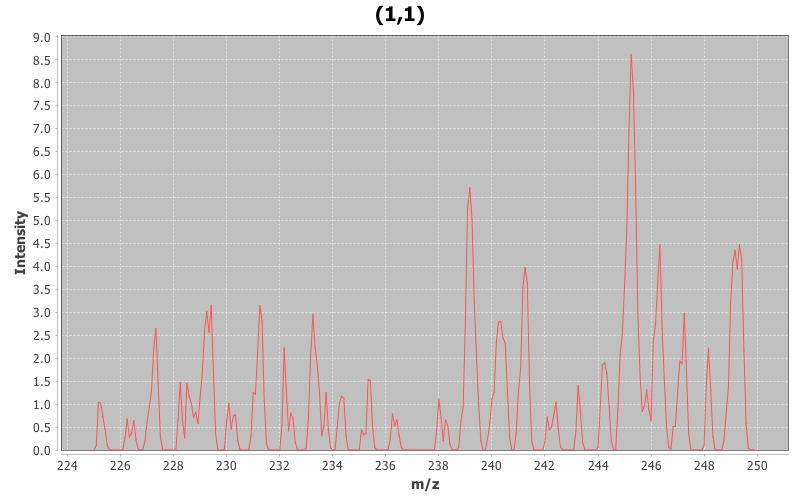
\includegraphics[scale=0.4]{./images/urinary_bladder_(1,1)_unprocessed.jpeg}
    \caption{An example of a Mass Spectrum (often called spectrum) sampled from pixel location (1,1) of a urinary bladder. This spectrum has a manually reduced maximum intensity, but is otherwise unprocessed. Data sourced from \url{https://ms-imaging.org/wp/imzml/example-files-test/} \cite{imzml.org}.}
    \label{fig:unprocessed_urinary_bladder_spectrum}
\end{figure}

\subsection{Mass to Charge Ratio}
We see from figure \ref{fig:unprocessed_urinary_bladder_spectrum} and the previous subsection, that we typically plot a spectrum as its intensity against the m/z or mass to charge ratio. Here we will briefly explain the mass to charge ratio. Mass to charge is the mass of the ion (m)
divided by the charge of the ion (z). We measure the mass to charge ratio in 
units of thomson (Th). However, it is typical for the units of measurement to be omitted.  
 
\subsection{A Brief History of Mass Spectrometry}
Here, in order to better explain and motivate MS, we briefly review it's short history. We typically associate MS as a field of chemistry, however it's beginnings are in physics. MS was invented "accidentally" by \textit{J.J.Thomson} at Cambridge University, whilst researching electricity transmission in gasses. In particular, \textit{J.J.Thomson} and his team were performing experiments to magnetically deflect cathode rays. Thomson won the 1906 Physics nobel prize for his work, as he discovered the electron. In the early 1900's, Thomson built the first mass spectrometer with his colleague Fancis Aston, which was used to measure the masses of charged atoms [\cite{history_of_ms_anal_chem}].

MS was heavily used in experiments on the atom only within physics until the 1940's, when Alfred Nier worked not only on Spectrometer machines, but on promoting the practice to other fields, and its popularity began to rise in other fields.

\subsection{A Practical Overview}
Here, we will take a general view as to how a Mass Spectrometer takes readings. Below, we can view the general parts of a mass spectrometer, this should help us visualize what a mass spectrometer does, which is discussed later in this section.

\begin{figure}
    \centering
    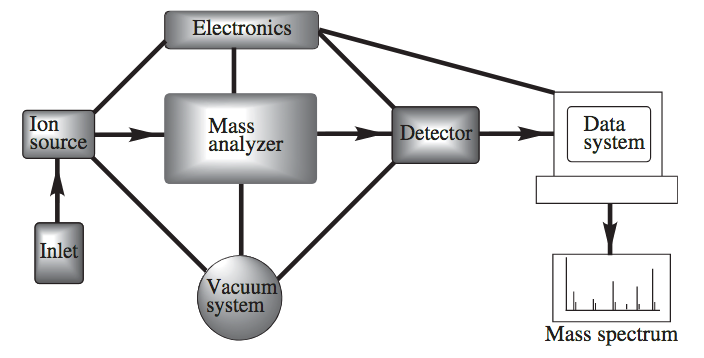
\includegraphics[scale=0.6]{./images/mass_spectrometry_process_diagram.png}
    \caption{Basic parts of a Mass Spectrometer, this is taken directly from "Fundamentals of Contemporary Mass Spectrometry" by Chhabil Dass \cite{fund_contemp_MS_book}}
    \label{fig:Parts_of_a_mass_spectrometer}
\end{figure}

Mass spectrometers typically have an inlet, which is used to introduce the analyte (sample) to take readings from, it transfers the analyte to the ion source. It is important that the inlet maintains the integrity of the sample. There is also an ionization source, which is used to produce ions from the analyte, it converts the sample into gas phase ions. 

The mass analyzer is used to separate the ions within the analyte, a mass spectrometer can have only one, or multiple mass analyzers. The spectrometer has a detector, which is used to count and amplify the abundance of ions which appear from the analyzer.

The mass spectrometer has an electronics component, which is used to control the execution of parts of the spectrometer. There is a vacuum system, which is used to maintain low pressures in the other components, in particular the ion source is kept at a very low pressure of approximately $10^{-4}$ - $10^{-8}$ torr \cite{fund_contemp_MS_book}. 

Lastly, the mass spectrometer has a data system, which is used to process the data. This can involve saving the data in a specific file format (eg mzML, imzML), or processing, and visualizing the spectra. Later on in this report, we will focus on the data processing side of \acrshort{ms}.

This is the general structure of a mass spectrometer, however many versions of spectrometers exist, and sometime combine certain elements of the spectrometer, in particular, mass analyzers and detectors are often combined.w

A typical mass spectrometer will use this array of components to create data on the analyte by the following steps. Firstly, ionization of the sample will occur, this converts the sample to a gas phase ionic species \cite{fund_contemp_MS_book}. This is done through the removal of an electron or the addition of a proton, which can separate the sample.

Next, the ions are separated by their m/z (mass to charge) ratio in the mass analyzer. Then, we fragment selected ions to be analyzed in a second analyzer. 

The ions that emerge from the final analyzer are measured by their abundance, and a detector converts this to electrical signals.

Finally, these signals can be processed, analyzed and then displayed on a screen for the user of the system.

\subsection{Why Mass Spectrometry?}
Now we have an understanding as to what mass spectrometry is, and how it works, we can discuss why it is so widely used, and why it has become irreplaceable to many fields of research and industry.

MS can be used successfully on many different types of sample, this ranges from analyzing single elements, to real world complex biological samples. MS is a stable means of quantitative analysis regardless of the properties of the sample, it can be used on solids, liquids and gases, volatile and non-volatile samples \cite{fund_contemp_MS_book}.

MS is an extremely sensitive tool, it is capable of discovering extremely small amounts of a molecule in the sample. In fact, MS has successfully detected molecules in the zeptomole amounts in a substance. For reference, a zeptomole is approximately 600 molecules of a substance.

%%% IDK IF THIS PARAGRAPH IS NEEDED, MIGHT BE UNNECESSARY FOR JUST A SUBSECTION.
Now we have a base understanding in the fundamentals of Mass Spectrometry, we can look at a typical format for storing MS data, and the more practical aspects of this report to do with software, and processing of spectra. 

% \subsection{Mass Spectrometry Imaging}
% TODO : Talk about how we have a spectrum and can image it and make ion images at each m/z.

% TODO : Create image of a spectrum, with a few m/z channel images to show MSI.

% \subsection{MALDI MS}
% TODO : Talk about MALDI - eg talk about the rat brain and how it goes from frozen cut up tissue section to a set of spectra? Is this worth doing?

\section{imzML File Format}
In this subsection, we will introduce how MS datasets can be stored after the experiments are done. Specifically, we look at imzML (Imaging Mass Spectrometry) file formats, which aims to provide a common and accessible means to store and share MS data.

imzML data storage relies on two distinct files, an XML file (with a .imzML extension) which stores metadata about the experiment, and a binary file which stores binary data from MS experiments. 

\begin{figure}[H]
    \centering
    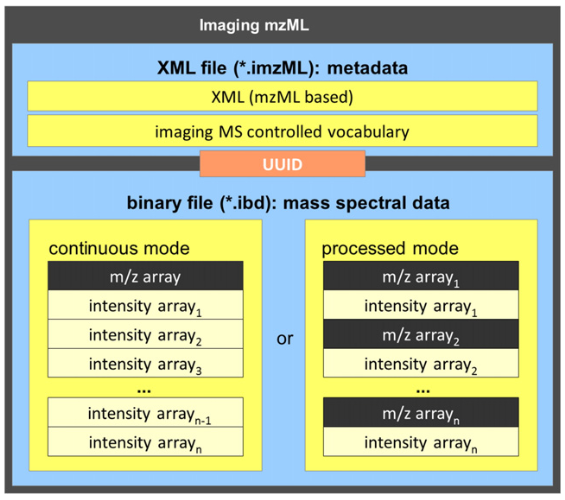
\includegraphics[scale=0.3]{./images/imzml_file_format.png}
    \caption{A diagram of the structure of imzML data. It shows well the two distinct files, .imzML and .ibd. It also documents how data can be stored in a continuous or processed format. This figure is sourced from \cite{imzml_file_article}}
    \label{fig:imzML_file_format}
\end{figure}

We note that imzML supports two styles of storing the binary data, processed and continuous. Continuous data is when the m/z values are constant for all spectra in the data, continuous data is clearly more efficient for storage. Whereas, processed is used when the m/z is not constant for all spectra, thus the m/z values must be stored with each set of intensity values. The UUID (universally unique identifier) is for linking these two files together, aiming to prevent the loss of information, which is of course possible, as the .ibd is unusable without the .imzML, and vice versa.

The imzML file format aims to bridge a gap between existing formats for gathering and processing Imaging Mass Spectrometry datasets, allowing software to interact with multiple formats of MS data through conversion to imzML.

MSI datasets can be extremely large, thus it is important that access of the data is fast and flexible. This is achieved by offset values stored in the XML which indicate the corresponding position of data in the binary file. Previous versions of MS data formats do not store the raw data in a seperate file, we have seen how this is critical for fast access. However, the XML file is made compatible with another MS data format, mzML 1.1, this was done in order to allow for easy conversion between imzML and this common format mzML. Below, we can view the performance between the two file formats.

\begin{figure}[H]
    \centering
    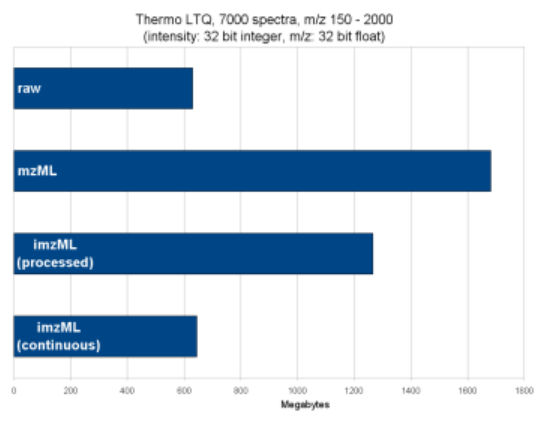
\includegraphics[scale=0.3]{./images/imzml_file_efficiency.png}
    \caption{A diagram plotting the storage space for different formats of imMzML, and mzML. We see that the processed imzML is roughly 30\% smaller than the mzML, and the continuous file is almost four times smaller \cite{imzml.org}.}
    \label{fig:imzML_mzML_efficiency_comparison}
\end{figure}

\section{KNIME}
We now take a step back from MS, and do some background research into the software platform that we have built our software plugin for the analysis of MS data in. We do this research to give the reader an understanding of the platform we used, which is Knime. 

KNIME - the Konstanz Information Miner is an open source software platform that is designed for easy, fast and modular access to data science. The software displays a GUI, which allows the user to interactively design a data processing workflow using "nodes." A "node" is an object within Knime, which performs some sort of data generation, readion, processing, or visualization. Knime is installed with an extensive repository of nodes, and offers easy access to community made nodes which can be downloaded within the Knime platform. Figure \ref{fig:knime_workbench_workflow_img} shows an image of the Knime workbench, with an example "workflow," which is simply a graph of connected nodes, more specifically, it is a direct acyclic graph. 

\begin{figure}[H]
    \centering
    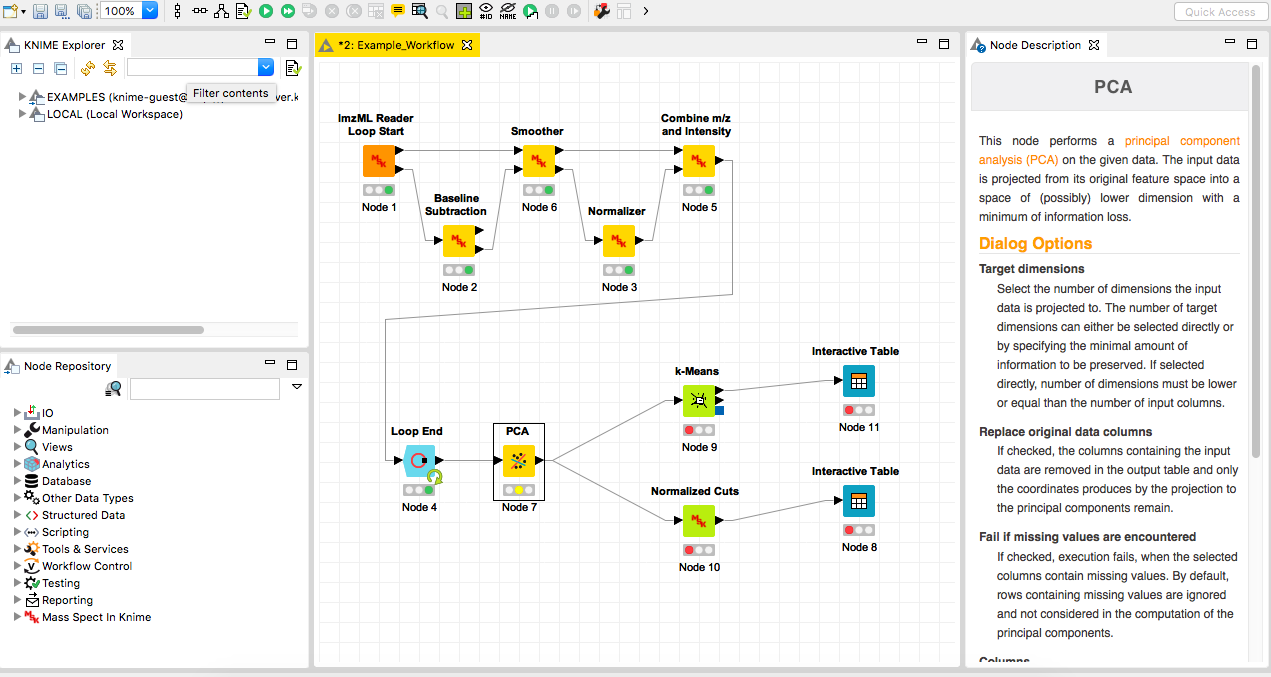
\includegraphics[width=\textwidth]{./images/knime_workbench_workflow_img.png}
    \caption{The KNIME workbench, with a workflow in the center of the figure. The right side of the figure displays the Node description of the currently selected node (PCA - Principal Component Analysis), which displays useful information about the selected node. On the bottom left is the node repository, which houses all nodes in this instance of KNIME, above the node repository is the KNIME explorer, a file explorer for the current workspace.}
    \label{fig:knime_workbench_workflow_img}
\end{figure}

KNIME was designed with three main aims \cite{KNIME_Basic_info}, firstly, it aims to be a visual, interactive framework, in which users easily drag and drop processing units (nodes) into their workflow. Next, it aims to be modular, in that nodes should typically not depend on each other, and processing should not be type specific. Finallly, Knime is aimed to be easily extensible. this is achieved through an extensive API \cite{KNIME_API_URL} for building and distributing new nodes.

KNIME is built on top of the Eclipse IDE in the programming language Java. Java is an extremely popular language with a very large community, is open source, and platform independent, thus aiding in Knime's goals of extensibility. 

\subsection{Data Structures}
\label{subsection:Background/KNIME/Data_Structures}
Nodes are connected with ports, which allow for nodes to be connected. More specifically, there are in-ports, which is for incoming data to that node, and there are out-ports, for data leaving that node. A node may only have one connection for each of its in-ports. However, it may have an arbitrary number of connections from any of its out-ports. This ensures consistency in what data is being used when executing a node, and it allows workflows to take many different paths.

Data within Knime is all wrapped in a class \texttt{DataTable}, which stores the data, and relevant metadata, including information about the column types, number of columns. Rows of data within the \texttt{DataTable} are stored as \texttt{DataRow} objects, each of which has an associated unique \texttt{RowKey}, which is a unique identifier for that row of data. Every \texttt{DataRow} must be the same length as the number of columns of the \texttt{DataTable}. We can access entries in the \texttt{DataTable} by iterating through \texttt{DataRow}'s, and then iterating through the \texttt{DataCell}'s making up each row. 

Knime's data structures are excellent for the purpose of this project because they use a powerful caching strategy, allowing parts of a \texttt{DataTable} to be stored in the hard drive when the table becomes too large\cite{KNIME_Basic_info}. This is useful due to the large nature of MS datasets. One drawback to Knime's data structures is that they require a running instance of Knime to work properly, which means some Knime code cannot be unit tested in the typical way, eg JUnit. 

\subsection{Node Development}
Despite Knime's extensive repository of existing nodes, it is often useful to build nodes for specific use cases. This requires the development of four java classes, and an \texttt{XML} file storing metadata about the node. The java classes for the new node must each extend one of the following, \texttt{NodeModel}, \texttt{NodeFactory}, \texttt{NodeDialog}, \texttt{NodeView}, and the \texttt{XML} file must have the same name as the class extending the \texttt{NodeFactory} \cite{KNIME_Basic_info}.

Here, we will briefly explain what each of these classes function is. Firstly, the \texttt{NodeModel} class is where the actual function of the node is executed, where incoming data is processed and an outgoing \texttt{DataTable} is created. Next, the \texttt{NodeDialog} class is used to create a basic GUI, which allows user the specify how they wish the node to execute, and change parameters for the node. The \texttt{NodeView} class specifies a GUI which is created upon execution of the node, and can be opened by the user. More than one View can be created when necessary, these are typically used to visualize results of exection in the node. The \texttt{NodeFactory} informs the Knime instance on how to use the node and what class to use to build the dialog, and view, and how many views there are.

\begin{figure}[H]
    \centering
    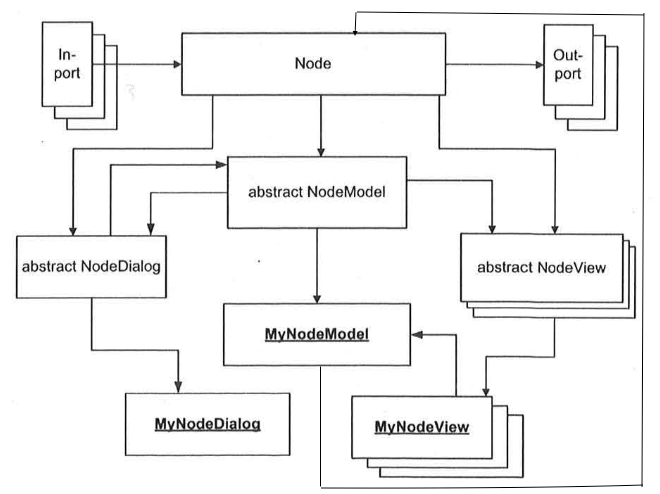
\includegraphics[scale=0.3]{./images/knime_data_structure.png}
    \caption{The class structure showing how a Knime node is created, we note that the NodeFactory is not considered in this. This is taken and edited from \cite{KNIME_Basic_info}}
    \label{fig:knime_node_class_structures}
\end{figure}

\subsection{NodeModel}
As we have seen the NodeModel stores the handling of incoming data, and creates a new \texttt{DataTable} to return. There are three methods in this class that stand out and are important for the processing of the node. The most important is the execute() method, which is called whenever the node is executed in Knime. This is the method which connects to the logic which is often implemented in other classes. The configure() method is an internal method which sets an expected \texttt{DataTableSpec}, which stores metadata on its respective \texttt{DataTable}, for the outgoing table which is created in the execute method. Lastly, the reset() method is executed when the reset button is pressed in Knime, and the node is in an executed state. Here, we can reset variables in the class and ensure the execute method can be called again.

\subsection{Meta nodes}
Meta nodes are a powerful tool and a special type of node in Knime which allows us to wrap parts of a workflow into a single node. This allows us to create more complicated workflows without the workflow becoming cluttered. It also allows for some consistency in workflows. For example if you wish a certain workflow to always have the same preprocessing workflow, wrapping this sub workflow in a meta node would ensure this. Knime has a wizard which allows nodes to be created with an arbitrary number of ports. 

%-----------------------------------------------------------------------
% SECTION : RESEARCH (LITERATURE REVIEW)
%-----------------------------------------------------------------------
\chapter{Research}
\label{chapter:Research}
In the beginning of this project, we spent some time researching existing software that has similar use cases to ours. In particular, we looked at Spectral Analysis by Alan M. Race et al. \cite{spectral_analysis_article} and MSIQuant by K{\"a}llback et al. \cite{MSI_QUANT_Article}. Mass Spectrometry datasets appear to be increasing in size with increases in technology, and the number of datasets used to analyze a sample are increasing, we notice immediately that both of these applications are built with the notion that they must handle large datasets. For the remainder of this chapter, we will discuss these applications.

\section{Spectral Analysis}
Spectral Analysis is a GUI based software that was developed in Matlab and aims to provide a common tool that can be used to preprocess and visualize MSI data in the imzML format that the community has decided as a common format for sharing MSI data. We learned that mass spectrometry instrunment vendors often provide software to analyze and visualize data, but they typically rely on proprietary data structures. This coupled with the lacking of industry standard preprocessing methods means that it is hard to compare data between different vendors and their machines. This is a strong argument for use of the imzML data format as most instrunment vendors provide tools for converting their proprietary formats to imzML \cite{spectral_analysis_article}.

Spectral analysis implements functionality for many different preprocessing methods, rebinning, smoothing, baseline correction, peak detection, datacube generation for memory efficient principal component analysis are all supported. There is a great focus on comparison of preprocesisng methods which led to us implementing many of the methods suggested in this work. This software also implements many multivariate analysis techniques, including principal component analysis, probabilistic latent semantic analysis, non-negative matrix factorisation. Not much software in MSI adds this implementation, however we chose to focus more on the preprocessing methods, but these would be grounds for interesting work in the future.

We learn that a lot of MSI software load full datasets into RAM before processing occurs, MSI data is typically very large and is rapidly increasing. This places a bottleneck on the hardware, and was usually solved by considering smaller amounts of data by limiting m/z channels or the number of pixels by a Region of Interest. This limits our understanding of the data, and Spectral Analysis provides memory efficient methods that require a single spectra in memory, which may only require memory in the KBs as opposed to a whole dataset which could require imemory in the GBs. This is something mentioned in both Spectral Analysis and MSIQuant, which is why we provide loop support in our application, so that we are required only $n\in \mathbb{N}$ spectra in memory at any given time, where $n$ is specified by the user. 

\begin{figure}
    \centering
    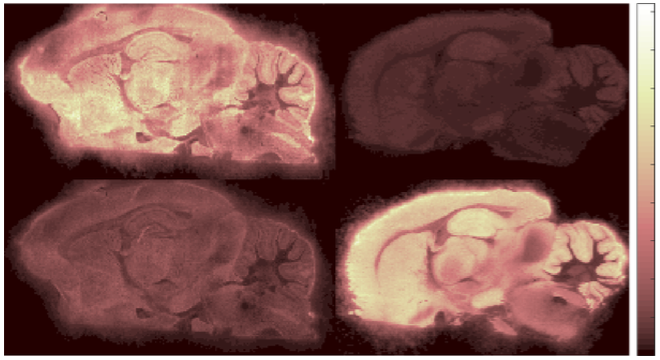
\includegraphics[width=0.6\textwidth]{./images/spectral_analysis_ion_images.png}
    \caption{Ion images generated in Spectral Analysis, taken from Spectran Analysis : Software for the Masses by Alan M. Race et al. \cite{spectral_analysis_article}. The colour scale used in these ion images is very good.}
    \label{fig:spectral_analysis_ion_images}
\end{figure}

Lastly, we see that Spectral Analysis is built with the aim of being extensible, allowing new processing methods to be added without needing an updated GUI. This is good software development practice and something that we have aimed to employ in our software, so that new processing methods can be added to the existing functionality. The software that we have implemented our extension in, Knime, is built with extensibility in mind, and aided us in building an extensible tool easily. However, we notice a drawback with Spectral Analysis, that is the choice of development environment. The application is built in Matlab, with some methods in C for efficiency, Matlab is closed source and perhaps contradicts the aim of extensibility, adding a barrier to extending the software. 
 
\section{MSIQuant}
Next we take a look at MSIQuant, which is another GUI based application which is built around the concept of handling large MSI datasts without storing the whole dataset in memory, and is also based on the use of the common MSI data format imzML. MSIQuant is capable of loading upwards of 50GB of imzML in seconds, and because it is based on the use of imzML, is also "manufacturer independent" \cite{MSI_QUANT_Article}. A key difference between these two applications is that MSIQuant loads the imzML binary data into its own data format, where as Spectral Analysis keeps the data in does not load the data into any other format. In MSIQuant, the data is loaded into two different modes, spectrum mode and image mode, where image mode is essentially the transpose of the spectrum mode. This novel approach to handling MSI data means that both spectra and ion images can be quickly generated, without having to iterate through all of the data in either case. We understand the benefits of this. However, for the purpose of our softwware implementation, we chose not to follow this route, as developing a new data format could be costly in time for this project. Perhaps, this would be good work for the future, to create a reader node in Knime that stores data in ion image format, as we currently store data in spectrum format. 

With respect to the processing of mass spectra, it is suggested that baseline correction methods and peak alignment algorithms are important for creating useful ion images. Baseline correction can be used to increase the accuracy of the signal to noise ratio, and peak alignment can be used to reduce the impact of mass shifts that occur during Mass Spectrometry experiments \cite{MSI_QUANT_Article}. While baseline correction methods is something that we focused heavily on, peak detection and alignment algorithms are something that we did not focus on, and would be a worthwhile functionality that we can add to our software in the future. We see that MSIQuant places a great emphasis on Regions of Interests, offering square, polygonal and elliptical ROI's. We see that there is a great focus placed on ion image processing in the software, this is perhaps too much for our software given the time constraints, but would be a good place to continue with further work.

\newpage
%-----------------------------------------------------------------------
% SECTION : SOFTWARE IMPLEMENTATION
%-----------------------------------------------------------------------
\chapter{Software Implementation}
\label{chapter:Software_Implementation}
In this chapter, we aim to provide a general introduction to the software implemented for this project. We will briefly introduce the algorithms that we have implemented in the nodes, but they will be looked at in greater detail in later parts of this report. 

\section{Mass Spectrometry In Knime Category}
Software plugins built for KNIME must be built into Java's archiving file, \texttt{.jar}, and then are placed in a specific subdirectory within the KNIME application. KNIME extensions can appear as a singular node, in which case the node just appears at the bottom of the repository. Typically, there will be multiple nodes in a single extension, thus KNIME allows larger extensions to appear with multiple "categories". A category is simply a collection of nodes, which can be stored in sub-directories. Notably,  This is the strategy that we have used for our extension. For a new KNIME extension to appear and be used, the application must restart. Once the application is opened, our software extension appears at the bottom of the node repository (see Figure \ref{fig:knime_workbench_workflow_img}), below the existing node extensions. Importantly, KNIME makes sure that groups of nodes within the repository do not interfere with one another, for example we can be assured that our nodes will not appear in the existing groups of nodes in the repository.

\begin{figure}[H]
    \centering
    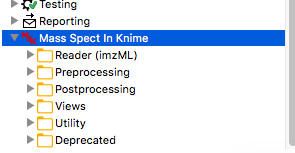
\includegraphics[scale=0.5]{./images/MSK_Node_Repository.png}
    \caption{Our KNIME software extension as it appears in the KNIME node repository below the existing categories, named "Mass Spect in Knime"}
    \label{fig:msk_node_repository_viewing}
\end{figure}

\section{Implemented Nodes}
As we see in figure \ref{fig:msk_node_repository_viewing}, our category has all implemented nodes separated into appropriate categories. Here, we will briefly introduce these categories and provide a list of all implemented nodes. We have a category "Reader" which stores all nodes used to load imzML data into KNIME. We also have a "Preprocessing" category, which stores nodes that we use to preprocess the data, for example reduce noise, subtract baseline and ensure a consistent m/z axis. We have a category "Postprocessing" which we use to store clustering methods that can be used on MSI data in Knime. We have a "Views" category which is used to store some nodes which implement some basic visualizations of MSI Data. There is a category of "Utility" nodes, which are used for table manipulations in Knime, that we require to do, but isn't supported allready in KNIME. Lastly, there is a "Deprecated" category of nodes, which we have included in order to document changes as the project has developed. Table \ref{table:Nodes_In_Our_Category} shows all nodes in their respective categories, we have omitted the deprecated category from this however, as they are not relevant here. 

% TABLE GENERATED HERE : http://www.tablesgenerator.com/latex_tables#
\begin{table}
    \centering
    {
        \renewcommand{\arraystretch}{1.4}
        \begin{tabular}{|l|lc|}
            \hline
            \multicolumn{3}{|c|}{\textbf{\underline{Mass Spectrometry in Knime}}}                                                                                   \\ \hline
        \multicolumn{1}{|c|}{\textbf{Category}} & \multicolumn{1}{c}{\textbf{Nodes}}  & \begin{tabular}[c]{@{}c@{}}\textbf{Algorithms}\\ \textbf{(if applicable)}\end{tabular} \\ \hline
        Reader (imzML)                 & imzML Reader               &                                                                      \\
                                       & imzML Loop Start           &                                                                      \\
                                       & imzML Processed Loop Start &                                                                      \\ \hline
        Preprocessing                  & Rebinning                  &                                                                      \\ \cline{2-3} 
                                       & Baseline Subtraction       & Minimum                                                              \\
                                       &                            & Median                                                               \\
                                       &                            & Morphological Operators                                              \\ \cline{2-3} 
                                       & Smoothing                  & Savitzky-Golay                                                       \\
                                       &                            & Moving Mean   \\
                                       &                            & Triangular Moving Mean
                                       \\ \cline{2-3} 
                                       & Normalization              & Total Ion Count (TIC)                                                \\
                                       &                            & Median                                                               \\
                                       &                            & Euclidean Norm                                                       \\ \cline{2-3} 
                                       & Image ROI                  & Rectangular ROI                                                      \\ \cline{2-3} 
                                       & Spectral Representations & Mean Spectrum \\
                                       & & Basepeak Spectrum \\
                                       \cline{2-3}
                                       & Limit m/z Range            &                                                                      \\ \hline
        Postprocessing                 & Self Organizing Maps (SOM)      &                                                                      \\ \cline{2-3} 
                                       & Normalized Cuts            & Lanczos Algorithm                                                    \\ \hline
        Views                          & Spectrum Viewer            &                                                                      \\
                                       & Spectrum Compare           &                                                                      \\
                                       & m/z Channel Viewer         &                                                                      \\
                                       & Cluster Viewer             &                                                                      \\ \hline
        \end{tabular}
    }
   
    \caption{Table listing all of the categories and their respective nodes that we have implemented in our Knime category, it also displays any algorithms associated with the node that we have used. We have however omitted the deprecated nodes.}
    \label{table:Nodes_In_Our_Category}
\end{table}

\section{Software Design}
Here, we will discuss the overall design of our system, and how we interface data between our nodes in KNIME's data structures. We aimed to design our nodes to be independent of each other, and to each perform one task only. For example, we could have our reader nodes combine certain preprocessing tasks while reading, however we felt it is more practical if each task is its own node, allowing the user to define the structure and order of their workflow. 

Our design relies on storing the m/z and intensity values of a spectra as rows in KNIME's \texttt{DataTable} data structure, and not as columns. The other option was to store spectra as columns. We chose to store spectra as rows because it is much more efficient, and KNIME's \texttt{DataTable} data structure is built to access rows, as opposed to columns, making access of values much easier. Furthermore, KNIME has better support in its existing node repository for data instances which are stored in rows. For example, the k-means clustering node in the repository, is built to store data instances as rows, and not columns. The drawback of this is that KNIME stores the column names and types in an array in memory, and hence this will likely be larger than if we stored as columns, as there are typically a lot of m/z channels stored. However, as we provide support to read in and process data in chunks, this should not have a large impact on our software.

Lastly, our nodes are designed such that before preprocessing has finished, the m/z and intensity values are stored seperately in different \texttt{DataTable}'s, and hance these nodes have two in and two out ports. We chose to do this so that the user can have complete control over the order of processing in the workflow. If we did not do this, then we would be required to rebin processed imzML data before doing any other preprocessing, otherwise exceptions would be thrown as rows would not be consistent in tables. Once preprocessed, we assume that the data can be combined into one \texttt{DataTable}, and hence combine the m/z and intensity tables before it can be visualized.

\subsection{Row Key Unique Identifier}
Due to the spatial nature of MSI data, it is important that we maintain the spatial location associated with each spectrum, if we do not know what pixel the spectrum came from after processing, the results will not be as meaningful. As we store spectra in rows of the \texttt{DataTable}, we require a unique String key for each row. Our software uses a row key in the form "$(x,y)$", where x is the location in the width of the image of the spectrum, and y is the location in the height of the image. We have created an object \texttt{KeyLogic} to handle this and allow for easy access and creation of these keys. Some nodes existing in the repository concatenate numbers to the row keys, in order to ensure uniqueness, our class ignores this and handles it regardless.

\subsection{Node Invariant}
All of our nodes aim to ensure this simple invariant, which is that the order in which rows are output from the node must be exactly the order that the rows were input to the node. This invariant can of course be broken during execution of the node, as long as it is repaired before finishing, as it is done when the nodes are multithreaded. This is important once the processing has finished, and perhaps we may wish to visualize the data, this ensures that the image is correct.

\section{Package Structure}
Here, we will briefly discuss the structure of java source code in our software implementation. Each node that we have implemented has its own package, we saw this as important to provide clear separation between java classes used for each node. That is, the package associated with each node will contain the following java classes, \texttt{NodeModel}, \texttt{NodeFactory}, \texttt{NodeDialog}, and if the node has a view a \texttt{NodeView}. Each package associated with a node also has the \texttt{NodeFactory.xml}, which is used to store usage guidelines for the node, and any important information about the node in markup. Lastly, each package has a \texttt{package.html}, which is used to store information about the package and where the logic for the node is found, typically this is where licenses for the node is located also.

As we have seen in previous sections, KNIME data structures require a running instance of KNIME in order to work. Hence, we chose to store all logic required for our nodes completely separate of any KNIME data structure, so there are separate packages for preprocessing, postprocessing, utility, and visualization logic implemented by the nodes. This allows us to more logically store the java classes, and to properly JUnit test them, without requiring a running instance of KNIME. 

\section{Multithreaded Design}
Mass spectrometry datasets can be extremely large, and seem to be increasing as sampling technologies become more sophisticated, thus it is important that we can optimise the processing of mass spectra. We do this by employing a multithreaded design at our preprocessing nodes. In the execute method for these nodes, we have a conditional such that if the number of rows in the incoming DataTable is greater than some $n \in \mathbb{N}$, a threadpool is created to concurrently process the spectra, otherwise the single main thread continues in execution of all spectra. As we have seen, each preprocessing node has an associated java class which stores the logic for the execution of the node. These logic classes all implement java's Runnable class to allow a thread pool to be created consisting of multiple executing preprocessing classes. Importantly, we must ensure that our node invariant remains true on return of the spectra from the node, so they are sorted before being added to the output table. Sorting has $O(\log n )$ complexity and may not be appropriate for very large amounts of data. However, this is suitable for our use case because we will typically not process a very large number of spectra per iteration.

\section{Supporting Information Document}
As this project consisted of some software engineering, we felt it was appropriate to create a supporting information document during the implementation of the software. There is a link to this document in section \ref{subsection:Appendix/Supporting_Information}. The main aim of this document is to store the functional requirements and test cases for the nodes. In this subsection, we will discuss our approach to software engineering, which is also discussed in the supporting information document.

\subsection{Software Engineering Practice}
During different phases of the project, we chose to alter our approach to software development. Before any software developemnt was performed, we chose to spend some time researching the Knime platform, and it's data structures. The initial phase of development involved an approach using rapid prototyping, aiming to get a few basic, working Knime nodes. The aim of this phase was to quickly learn in a practical sense how the Knime framework can be extended. This phase of rapid prototyping lasted for roughly 2 weeks, after which an agile approach was taken. We used the concept of sprints, by which we would make a list of tasks that we would aim to complete each week between meetings with my supervisor Iain Styles. For example, the first sprint was one week long, in which we aimed to implement nodes to be used for the reading of imzML data into Knime. Sometimes these sprints were completed on time, and others we had to dedicate more time to them, in particular the implementation of the Normalized Cuts algorithm. We aimed to complete sprints on nodes which had the most important functionality and were not dependent on other sprints first. For example, it was important that we completed reader nodes before building any nodes for processing or visualizations. 

Overall, I believe that this approach to was successful and appropriate for the project, as we needed to spend some time learning the development cycle of a Knime node. In hindsight, I believe focusing only on an agile approach would have been superioor. I believe that the rapid prototyping phase was in the grand scheme not as efficient as it relied on disposing of some source code and nodes.

\subsection{Requirements Documentation}
Our system is unique compared to a typical software project, as it involves the implementation of many small pieces of software, as opposed to a single large software. It is for this reason that we list the functional requirements for each individual node as its own independent system, where typically we may have a large requirements document. Next, we give an example of the requirements from a single node, but we can find similar for other implemented nodes in the supporting information document.

% Numbered list of requirements
\begin{titlemize}{ImzML Reader Loop Start Node Functional Requirements :}
    \item The node must read in imzML datasets by spectrum.
    \item The node must have 0 input ports.
    \item The node must have 2 output ports.
    \item The node should allow the user to specify how many spectra to output per chunk.
    \item The node must output the m/z values for a given spectrum in a row in the DataTable in output port 1.
    \item The node must output the intensity values for a given spectrum in a row in the DataTable in output port 2.
    \item The node must pair the m/z values and the intensity values for a given spectrum.
    \item The node could have a view displaying meta information about the imzML dataset.
    \item The node must have only one File Chooser, for the user to input the path to the .imzML file located.
    \item The node must not have a File Chooser for the .ibd file.
    \item The node must only accept the .imzML file as input, such that the .ibd file is in the same directory and has the same name as the .imzML file.
\end{titlemize}

\subsection{Test Plan}
As we have seen in section \ref{subsection:Background/KNIME/Data_Structures}, Knime data structures require a running instance of Knime in order to work properly. This results in some difficulty when it comes to testing, and forces us to take two separate approaches to testing. The logic behind most nodes doesn't require the use of Knime data structures, and thus we unit test those classes using JUnit 4. As for the Knime nodes, we test those using the Knime testing framework. The Knime testing framework involves a category of nodes that are installed into the node repository, and can be used to create test workflows. The node that we are interested in using is the "Table Difference Checker", which has two in ports, and simply tests for differences in the incoming \texttt{DataTable}'s. If the values in the tables, and the meta information about the tables are the same, it executes correctly, and fails otherwise. In order to create a test workflow, we create a series of mini workflows, which have an expected and actual table input to the "Table Difference Checker". The testing framework allows us to automate the testing workflows, by introducing a "Run as test workflow" button in Knime, which automates the running of all testing framework nodes, and spawning a user interface with information on passed and failed tests, much like we see with JUnit test in Eclipse. As with the functional requirements for nodes, we treat the nodes as separate systems and have independent sets of tests and a test workflow for respective nodes. 

% Please add the following required packages to your document preamble:
% \usepackage[normalem]{ulem}
% \useunder{\uline}{\ul}{}
\begin{table}
\begin{adjustbox}{width=1\textwidth}
\small
{  \renewcommand{\arraystretch}{1.4}
\begin{tabular}{|l|l|l|l|l|}
\hline
{\ul \textbf{Index}}                                       & {\ul \textbf{Test}}                                                                       & {\ul \textbf{Expected}}                                                                               & {\ul \textbf{Actual}}                                                                       & {\ul \textbf{Result}}                             \\ \hline
\textbf{0}                                                 & Contained Directory                                                                       & Reader (imzML)                                                                                        & Reader (imzML)                                                                              & Pass                                              \\ \hline
\textbf{1}                                                 & Node Name                                                                                 & "imzML Reader Loop Start"                                                                             & "imzML Reader Loop Start"                                                                   & Pass                                              \\ \hline
\textbf{2}                                                 & Node Icon                                                                                 & Main MSK Icon                                                                                         & Main MSK Icon                                                                               & Pass                                              \\ \hline
\textbf{3}                                                 & Ports                                                                                     & 0 input, 2 output                                                                                     & 0 input, 2 output                                                                           & Pass                                              \\ \hline
\textbf{4}                                                 & Node Colour                                                                               & Orange (Source)                                                                                       & Orange                                                                                      & Pass                                              \\ \hline
\textbf{5}                                                 & Has Dialog                                                                                & True                                                                                                  & True                                                                                        & Pass                                              \\ \hline
\textbf{\begin{tabular}[c]{@{}l@{}}.\\ .\\ .\end{tabular}} & \begin{tabular}[c]{@{}l@{}}\textbf{.}\\ \textbf{.}\\ \textbf{.}\end{tabular}                                         & \begin{tabular}[c]{@{}l@{}}\textbf{.}\\ \textbf{.}\\ \textbf{.}\end{tabular}                                                     & \begin{tabular}[c]{@{}l@{}}\textbf{.}\\ \textbf{.}\\ \textbf{.}\end{tabular}                                           & \begin{tabular}[c]{@{}l@{}}\textbf{.}\\ \textbf{.}\\ \textbf{.}\end{tabular} \\ \hline
\textbf{11}                                                & \begin{tabular}[c]{@{}l@{}}Dataset = d\_1\\ N = 15\\ number of output rows\end{tabular} & \begin{tabular}[c]{@{}l@{}}9 in port 0\\ 9 in port 1\end{tabular}                                     & \begin{tabular}[c]{@{}l@{}}9 in port 0\\ 9 in port 1\end{tabular}                           & Pass                                              \\ \hline
\textbf{12}                                                & \begin{tabular}[c]{@{}l@{}}Dataset = \\ "NotAFile.imzML"\end{tabular}                     & \begin{tabular}[c]{@{}l@{}}Execute fails, popup\\ frame appears \\ "File doesn't exist".\end{tabular} & \begin{tabular}[c]{@{}l@{}}Execute fails, popup\\ frame appears as\\ expected\end{tabular}  & Pass                                              \\ \hline
\textbf{13}                                                & \begin{tabular}[c]{@{}l@{}}Dataset = \\ "NotImzML.html"\end{tabular}                      & \begin{tabular}[c]{@{}l@{}}Execute fails, popup\\ frame appears "Not imzML"\end{tabular}              & \begin{tabular}[c]{@{}l@{}}Execute fails, popup\\ frame appears as \\ expected\end{tabular} & Pass                                              \\ \hline
\end{tabular}
}
\end{adjustbox}
\label{table:Test_Plan_Table}
\caption{Table containing some of the tests for the node "ImzML Reader Loop Start node", we have omitted the tests 6-13. The first few are are split between cosmetics and functionality. Then after that we have tests that are based more around the functionality of the node.}
\end{table}

\section{Deprecated Nodes}
There are a number of nodes that we have decided to label as deprecated, due to design decisions being made after/during their development. The majority of these nodes are for reading imzML data in different fashion, that we decided didn't fit the need of the project. Typically, these nodes would be labeled as deprecated in the \texttt{plugin.xml} for our node extension, and would not appear within KNIME. However, we have decided to leave them in the project, to document how the project has evolved over time, and shows that it is possible to load the data into KNIME in more ways than we have done in our Reader category. 

%-----------------------------------------------------------------------
% SECTION: Reading imzML
%-----------------------------------------------------------------------
\chapter{Reading imzML}
For our software, we are required to load imzML data into KNIME, and we have a category of nodes built for this, which we will discuss in this section.
The "Reader (imzML)" category provides nodes for reading imzML data into KNIME's \texttt{DataTable} data structure. Our software provides support for both continuous and processed imzML, each of which requires the use of their respective nodes. Also, there is support for reading in imzML in chunks of data of size $n \in \mathbb{N}$ spectra per chunk, as specified by the user, and support for reading the whole imzML dataset into a \texttt{DataTable}.

Parsing imzML was not in the scope of this project, and so we use imzMLConverter \cite{imzMLConverter_article} to do this. It provides java classes for parsing imzML into java objects, notably \texttt{ImzML} and \texttt{Spectrum} objects. All of the reader nodes rely on the class \texttt{imzMLWrapper} which wraps the imzMLConverter objects into java's \texttt{Iterator}, to allow us to quickly and easily iterate through \texttt{Spectrum} objects in the file, and allowing quick access of the Spectrum's m/z array and intensity array.

\begin{figure}[H]
    \centering
    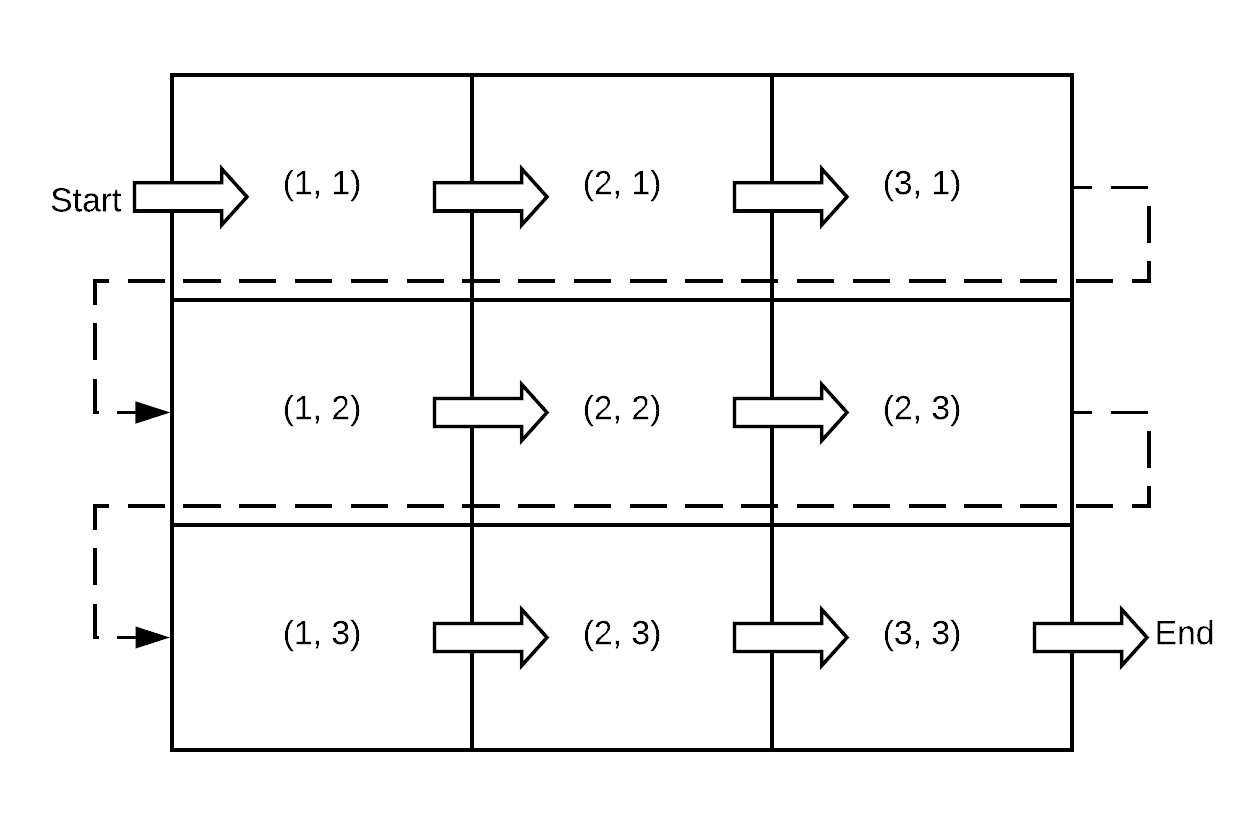
\includegraphics[scale=0.2]{./images/imzMLReading.png}
    \caption{Example of how we might visualize the spatial coordinates of an imzML dataset which has a width and height of 3, and how we iterate through all the pixel values, and their associated spectra.}
    \label{fig:imzML_reading_visualization}
\end{figure}

Above we see a visualization of how we iterate through the pixels of an imzML dataset to access their associated spectra. Specifically, we access each pixel row at a time, and when the row is empty, we access the first pixel in the row. The Iterator is finished when there is no next row to iterate over.

\section{Loop Support in Knime}
Two of the three nodes that we have implemented for reading in imzML are Knime Loop Start nodes. In order for them to work correctly, they must be paired with one of the following two nodes that are found in the node repository, "Loop End" or "Loop End (2 ports)". If we use the loop end node with 2 ports, then our m/z and intensity tables will not yet be combined, however if we use the single port loop end node our data must be combined using the "Combine m/z and Intensity" node that we have implemented. Figure \ref{fig:loop_start_reader_nodes} displays how we might build a workflow using the loop nodes, and metanodes which encapsulate a preprocessing pipeline.
In order to implement a Loop Start node, the node's respective NodeModel must implement the Knime interface for LoopStartNodeTerminator and overide the method terminateLoop(). Once, the execute() method finishes executing, terminateLoop is called, and if it returns false, the node will be finished executing, otherwise, it will call the execute() method once the connected Loop End node has finished execution. We note a drawback of this design is that we can only have one connected Loop End node for any Loop Start node, otherwise the workflow will not execute properly. 

\begin{figure}[H]
    \centering
    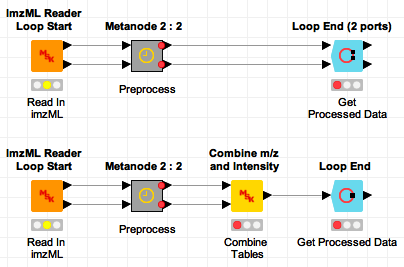
\includegraphics[width=0.8\textwidth]{./images/Loop_Start_Reader_Nodes.png}
    \caption{Example of two workflows that bout utilise the "imzML Reader Loop Start node" and preprocess data in their respective metanodes. The top workflow utilises a Loop End with 2 ports, and the bottom utilises a Loop End with 1 port.}
    \label{fig:loop_start_reader_nodes}
\end{figure}

%-----------------------------------------------------------------------
% SECTION : MASS SPECT PREPROCESSING
%-----------------------------------------------------------------------
\chapter{Mass Spectrometry Preprocessing}
We can represent a spectrum which has not been processed with the following equation, provided by \cite{alan_race_phd_thesis}.

\begin{equation}
    f(t) = \beta(t) + N \cdot S(t) + \epsilon(t),
    \label{equation:mass_spectrum_equation}
\end{equation}

where $f$ represents the observed, raw spectrum. $\beta$ represents a baseline, $S$ refers to the actual spectrum given by the sample. $N$ is a normalization factor. Lastly, $\epsilon$ represents a noise which refers to small, local fluctuations in the signal. These artefacts can originate from the machine used to collect the data, and from the nature of the sample, as is often the case with complex biological samples. We preprocess the data to limit the impact that these artefacts will have on images, and the quality of experiments on the data later down the workflow, and ideally we wish to isolate the original signal $S(t)$. In this chapter, we will state and discuss the preprocessing methods that we have implemented into our Knime extension. 

\section{Rebinning}
We feature a node which aims to ensure a consistent m/z axis among all spectra in a dataset, by fitting all spectra into a new m/z axis, this is particularly important for Knime, as all rows must have the same length. This is especially useful when we have to load processed data into Knime. It makes use of two algorithms based on Alan M. Race's thesis \cite{alan_race_phd_thesis}, the first takes a minimum m/z, maximum m/z, and a bin size, and uses these to calculate a new m/z axis, which we then fit all spectra to.

%Print rebin1
    \begin{algorithm}
    
        \label{alg:rebin1_generate_new_axis}
        \caption{Generate a new m/z axis, the first step in rebinning the data.}
        
        \begin{algorithmic}
           
            \Require $min, max, \delta \in \mathbb{R}$. $min$ and $max$ are the minimum and maximum values in the new m/z. $\delta$ is the bin size.
            
            \Ensure $M_{rebin}$ - the new m/z array.
           
            \Procedure{GenerateNewMZAxis}{$min, max, \delta$}
            
            \If{$\delta \leq 0$}
                \State \textbf{print} "Invalid bin size $\delta$"
                \State \textbf{throw} Exception
            \EndIf

            \State $n \gets \lceil (max - min) / \delta \rceil + 1$
            \State Initialize array $M_{rebin}$ of length n
            
            \For{$i := 0$ \textbf{to} $n-2$}
                \State $M_{rebin}[i] \gets min + i \cdot \delta$
            \EndFor
            \State $M_{rebin}[n-1] \gets max$
            \State \textbf{return} $M_{rebin}$
            \EndProcedure
        \end{algorithmic}
    \end{algorithm}


Once the new m/z axis has been calculated, we are ready to fit the spectra to this new m/z axis. For each bin in the new spectrum, we assign a value that is calculated by summing points which fall in a close proximity to the new bin, in the old m/z axis. By close proximity, we refer to any point which is less than half the new bin size distance away. 

% Print rebin2
    \begin{algorithm}
        \caption{Rebin a Spectrum to fit a new m/z axis.}

        \begin{algorithmic}
        
            \Require A Spectrum $S$ with corresponding m/z array $M$, the new m/z axis $M_{rebin}$ and the bin size of $M_{rebin}$, $\delta$.
            \Ensure $S_{rebin}$ - rebinned Spectrum array.
            
            \Procedure{RebinSpectrum}{$M, S, M_{rebin}, \delta$}
            
            \State $j \gets 0$
            \State $h \gets \delta / 2$
            \State $L \gets $ length of the array $M_{rebin}$
            \State Initialize a new Array $S_{rebin}$ of length $L$.
            \State $newMin \gets M_{rebin}[0]$
            \State $newMax \gets M_{rebin}[L-1]$
            
            \For{$i := 0$ \textbf{to} Length of array $S$}
                \If{$M[i] < newMin$}
                    \State \textbf{continue}
                \EndIf
                
                \If{$M[i] > newMax$}
                    \State \textbf{break}
                \EndIf
                
                \State $t_1 \leftarrow M[i] - h$;
                \State $t_2 \leftarrow M[i] + h$;
                
                \While{$j < L \&\& M_{rebin}[j] < t_1$}
                    \State $j++$
                \EndWhile
                
                
                \If{$j < L \&\& S_{rebin}[j] < t_2$}
                    \State $S_{rebin}[j] += S[i]$;
                \EndIf
            \EndFor
            \State \Return $S_{rebin}$.
            \EndProcedure
        \end{algorithmic}
    \end{algorithm}


Figure \ref{fig:rebinned_spectra} displays the effects of rebinning a spectrum from a urinary bladder with varying bin sizes.

% Here is the subfigure of rebinned spectra.
\begin{figure}
    \centering
    \subfloat[Raw Spectrum][Raw Spectrum]{
    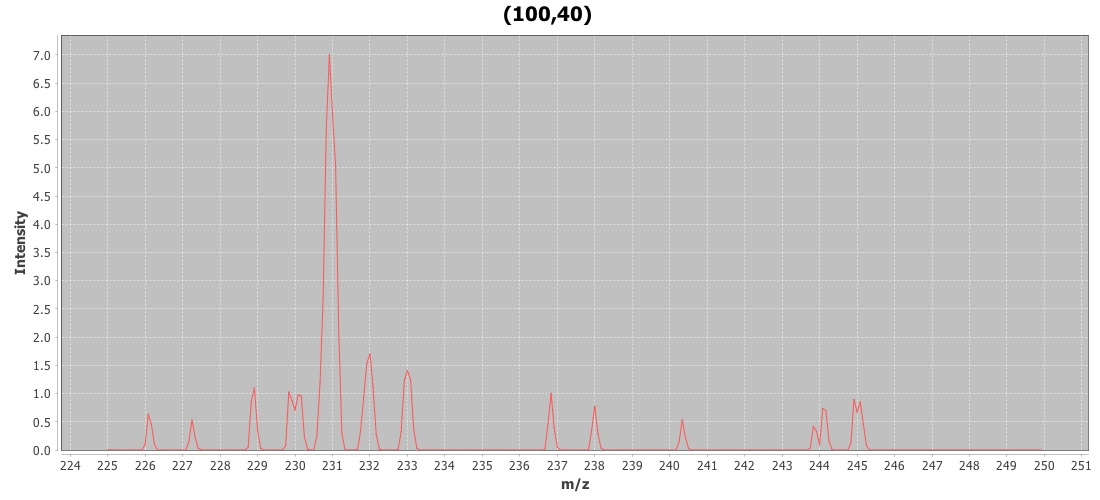
\includegraphics[width=0.56\textwidth]{./images/rebin/(100,40)_urinarybladder_raw.jpeg}
    \label{fig:rebinned_spectra_raw}}
    
    \subfloat[Rebinned with small bin size 0.05][Rebinned with small bin size 0.05]{
    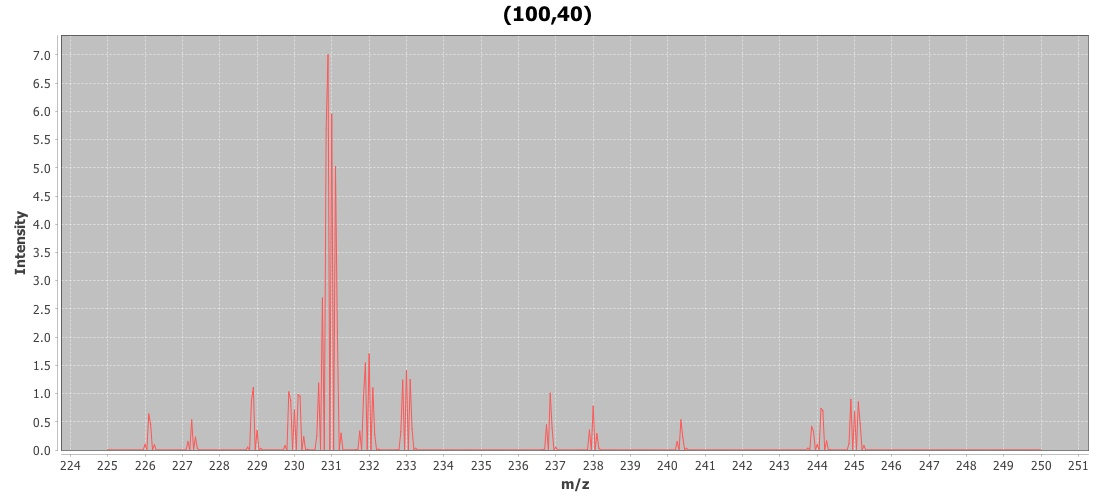
\includegraphics[width=0.56\textwidth]{./images/rebin/(100,40)_urinarybladder_binsize0-05.jpeg}
    \label{fig:rebinned_spectra_0.05}}
   
    \subfloat[Rebinned with medium bin size 0.5][Rebinned with medium bin size 0.5]{
    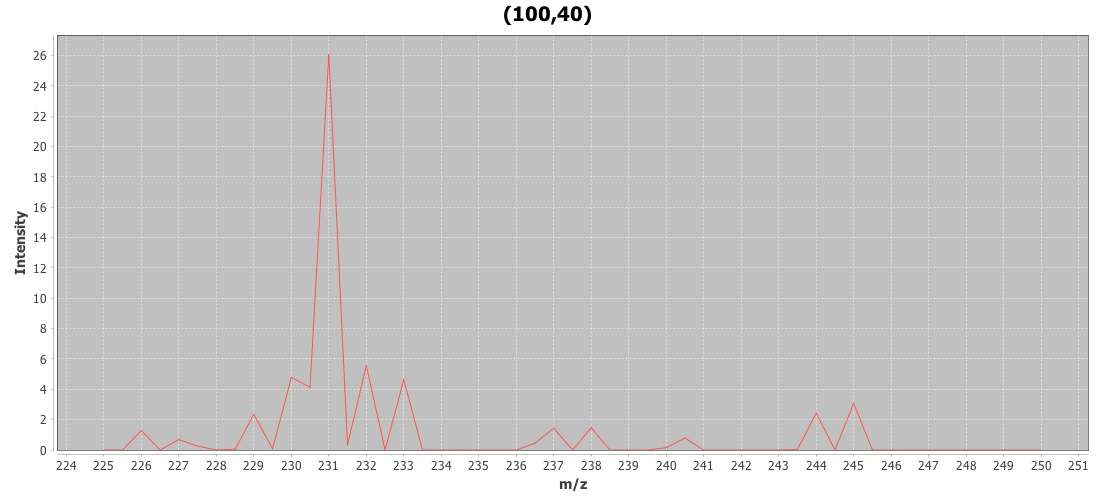
\includegraphics[width=0.56\textwidth]{./images/rebin/(100,40)_urinarybladder_binsize0-5.jpeg}
    \label{fig:rebinned_spectra_binsize0.5}}
    
    \subfloat[Rebinned with large bin size 1][Rebinned with large bin size 1]{
    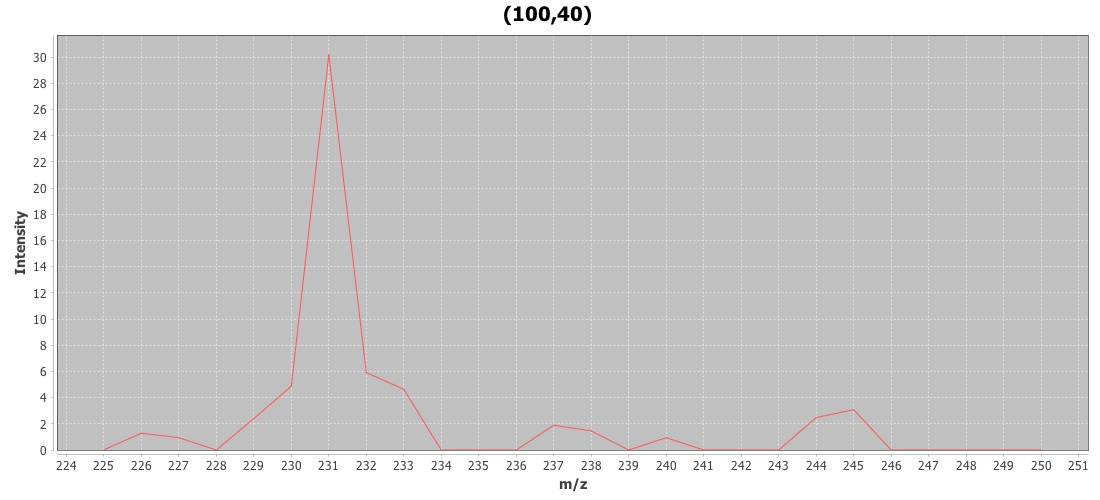
\includegraphics[width=0.56\textwidth]{./images/rebin/(100,40)_urinarybladder_binsize1.jpeg}
    \label{fig:rebinned_spectra_binsize1}}
    
    \caption{The effect of our rebinning algorithm on a spectrum taken from a urinary bladder dataset, with pixel location $(100, 40)$, sourced from \url{https://ms-imaging.org/wp/imzml/example-files-test/} \cite{imzml.org}. We show the raw spectrum, a very small bin size, a bin size which doesn't affect too much, and a large bin size. All of these were rebinned with minimum and maximum m/z equal to 225 and 250 respectively.}
    \label{fig:rebinned_spectra}
\end{figure}

As seen in Race's thesis \cite{alan_race_phd_thesis}, we see that when the bin size is very small with respect to the original bin size, see \ref{fig:rebinned_spectra_0.05}, we can introduce artefacts in the form of zeros in between peaks in the original spectrum. This occurs when a new bin appears too far away from any of the original bins, and thus nothing is added. If the bin size is large with respect to the original bin size, see \ref{fig:rebinned_spectra_binsize1}, then the peaks in the spectra can be distorted, and some peaks even combined, however the spectrum is also denoised. In the medium bin size case, see \ref{fig:rebinned_spectra_binsize0.5}, we see more of the original features, however, if we chose a smaller bin size, more features are kept.

Lastly, with regards to computational efficiency, we note that if a particularly small bin size is chosen, then the number of elements in the arrays storing the spectra can be greatly increased. Thus this has effects on computational efficiency both during the rebinning stage and later on down the workflow. This also effects memory, however, we can simply process less spectra at any given time, even a single spectra, thus memory efficiency is not a problem here. 

\section{Baseline Correction}
Baseline correction is used to limit the effect of $\beta(t)$ in equation \ref{equation:mass_spectrum_equation}, which represents amplified intensities, typically occurring in areas of low intensity, and low m/z, while still retaining information about the peaks in intensity. This amplified intensity is usually the result of chemical noise in the sample, but the instrument used to collect data also impacts the type of baseline present. We have implemented a node which provides support for four methods of baseline subtraction. The first two methods rely on estimating the baseline using a moving mean or a moving median, the remaining two methods rely on mathematical morphological operators dilation and erosion to estimate the baseline. All of these baseline estimation algorithms are all based on a moving window. Our node outputs both the estimated baselines for all spectra, and the original spectrum take away the estimated baseline. 

The first step in our baseline correction workflow is to estimate the baseline $B$, then we subtract the baseline from the spectrum by the following, where $S_{new}$ refers to the new Spectrum after the baseline has been subtracted, $S_{old}$ is the original spectra, and $B$ is the estimated baseline. 

\begin{equation}
    S_{new}[i] = S_{old}[i] - B[i],
    \label{eqn:subtract_baseline}
\end{equation}

We of course calculate this for every valid $i$ in the array $B$, which is the same length as the other arrays $S_{new}$ and $S_{old}$.

\subsection{Minimum and Median}
The simplest of our baseline estimation methods calculate the minimum and median of a symmetric window around every point in the spectrum, using the following equations,

\begin{equation}
    B[i] = min\{ S[i-k], S[i-k+1], \dots , S[i], \dots S[i+k-1], S[i+k] \}, 
    \label{eqn:minimum_baseline_estimation}
\end{equation}

\begin{equation}
    B[i] = median\{ S[i-k], S[i-k+1], \dots , S[i], \dots S[i+k-1], S[i+k] \}.
    \label{eqn:median_baseline_estimation}
\end{equation}

where $k \in \mathbb{N}$ is the distance the window extends in either direction.

\subsection{Tophat}
A more sophisticated baseline estimation algorithm called the Tophat, draws on theory which was initially proposed for image analysis, mathematical morphology, but has seen significant use in signal processing. The Tophat relies on two operators, erosion denoted by $\ominus$ and dilation denoted by $\oplus$. There are general definitions of these operators, however we define the version which can be applied to MSI data below \cite{baseline_morphology_paper}.

\begin{definition}[Erosion and Dilation]
    Given a spectrum $S$ and a structuring element $B$ that is a symmetric interval around zero, the erosion $\epsilon$ of $S$ with respect to $B$ is given by
    
    \begin{align}
        \epsilon_{B}(S)(x)      &= (S \ominus B) (x),\\
                                &= \min_{b \in B} \{ S(x + b), \}
    \end{align}
    for all values x that are in the spectrum S. Similarly, we can define the dilation $\delta$ by
    
    \begin{align}
        \delta_{B}(S)(x)    &= (S \oplus B) (x),\\
                            &= \max_{b \in B} \{ S(x + b), \}
    \end{align}
    for all values x that are in the spectrum S.
    \label{defn:erosion_and_dilation}
\end{definition}

We can view the erosion as a moving minimum, and the dilation as a moving maximum. If we combine these two operations we get the operations called opening and closing, we are only concerned with the opening for baseline subtraction.

\begin{definition}
    The morpohological opening $\gamma$ is an erosion followed by a dilation. 
    
    \begin{align}
        \gamma_{B} (x)      &= \delta_B(\epsilon_B(S))(x),\\
                            &= ((f \ominus B) \oplus B ) (x).
    \end{align}
\end{definition}

Combining the above, we are left with the tophat operator for baseline subtraction. The Tophat operator $\rho$ is the spectrum $S$ subtracted by the opening.

\begin{equation}
    \rho (S) = S - \gamma(S).
\end{equation}

\subsection{Optimal Tophat for Raman Spectroscopy}
Here, we look at another method of baseline subtraction using morphological operators which was suggested by Rosanna Perez-Pueyo et al \cite{baseline_raman_morphology_optimal_tophat}, for use on Raman spectroscopy data. Raman spectroscopy is another analytical technique used in the field of chemistry for understanding the chemical composition of samples. The output, as with MS, is a signal, except we plot the intensity against the wavenumber ($cm^{-1}$). There has been some literature suggesting that Raman spectroscopy can be used together with MS to further reinforce results in MS, more specifically, the presence of analytes in the samples \cite{combine_raman_spectroscopy_ms}.

The method of estimating the baseline is by taking the minimum of the two following operations,

\noindent\begin{minipage}{.5\linewidth}
    \begin{equation}
        \gamma (S),
    \end{equation}
    \end{minipage}
    \begin{minipage}{.5\linewidth}
    \begin{equation}
        \gamma^{'} (S) = \frac{ \delta[\gamma(S)] + \epsilon[\gamma(S)] }{ 2 }.
    \end{equation}
\end{minipage}

\subsection{Experiments}
We perform some experiments in order to test the validity of these baseline subtraction methods and to test whether specific methods would perform better on specific types of baseline. We perform these experiments on the whole of the urinary bladder dataset \cite{imzml.org}, as it has a variety of different spectra, that have peaks in varying areas in the m/z ranges. For each spectrum, we artificially add a baseline to the spectrum, and then perform one of the correction algorithms on the spectra. We then proceed to calculate the Euclidean distance between the original raw spectrum, and the spectrum which has has the artificial baseline removed. We then calculate the mean Euclidean distance over the whole dataset, a minimum and a maximum, and we have built the table \ref{table:Baseline_Experiments.} to display these results. The synthetic baselines that we have added to the dataset include the addition of a constant value, a decreasing linear function, a polynomial function, and a logarithmic function. Note that in the majority of these synthetic baselines, we have added the greatest level of baseline at the smaller m/z values, as typically baseline values are inflated at lower m/z values. 

We note that the dataset we are using has a width of 180 pixels and a height of 90 pixels, thus the total number of spectra considered is 16200. The m/z ranges from 225 to 250 with 300 channels. So the baselines that we have added have had to take this into consideration, the equations that we have added are listed below.

\begin{itemize}
    \item \textbf{Constant : } $B[i] = 5$,
    \item \textbf{Linear : } $B[i] = -\frac{13}{5}i + 600$,
    \item \textbf{Polynomial : } $B[i] = -0.1(i - 235)^2 + 7)$,
    \item \textbf{Logarithmic : } $B[i] = \ln(-i + 245)$,
\end{itemize}

for every valid index $i$ in the spectrum such that $B[i] \geq 0$.

If we take a loot at table \ref{table:Baseline_Experiments.}, we see that the success of the baseline correction depends on a multitude of factors, including the window size, and the type of baseline that was added. We see that for a constant baseline, the best results were achieved with minimum baseline subtraction, as we might expect, in fact if the window size spanned the whole dataset, we would get a 0 value for every spectrum. However, we notice that for the other baselines that have been added, the results are not as good for minimum baseline subtraction. In fact, the mathematical morphological operators work quite well, and typically achieve the best mean results.

% Please add the following required packages to your document preamble:
% \usepackage{multirow}
% \usepackage[normalem]{ulem}
% \useunder{\uline}{\ul}{}
\begin{table}[]
\centering
\begin{tabular}{|l|l|l|l|l|l|}
\hline
\multicolumn{6}{|c|}{{\ul \textbf{Baseline Correction Experiments}}}                                                                                                                                                                                                                                                                                                                                                    \\ \hline
\textbf{\begin{tabular}[c]{@{}l@{}}Baseline\\ Type\end{tabular}}          & \textbf{\begin{tabular}[c]{@{}l@{}}Window\\ Size\end{tabular}} & \textbf{Minimum}                                                & \textbf{Median}                                                  & \textbf{Tophat}                                                  & \textbf{\begin{tabular}[c]{@{}l@{}}Optimal \\ Tophat\end{tabular}} \\ \hline
\multirow{3}{*}{\begin{tabular}[c]{@{}l@{}}Constant\\ Shift\end{tabular}} & 3                                                              & \begin{tabular}[c]{@{}l@{}}6.932\\ 0.0\\ 422.969\end{tabular}   & \begin{tabular}[c]{@{}l@{}}10.811\\ 0.0\\ 623.744\end{tabular}   & \begin{tabular}[c]{@{}l@{}}9.523\\ 0.0\\ 579.391\end{tabular}    & \begin{tabular}[c]{@{}l@{}}8.495\\ 0.0\\ 534.285\end{tabular}      \\ \cline{2-6} 
                                                                          & 7                                                              & \begin{tabular}[c]{@{}l@{}}1.583\\ 0.0\\ 119.376\end{tabular}   & \begin{tabular}[c]{@{}l@{}}8.108\\ 0.0\\ 479.862\end{tabular}    & \begin{tabular}[c]{@{}l@{}}3.399\\ 0.0\\ 237.292\end{tabular}    & \begin{tabular}[c]{@{}l@{}}2.354\\ 0.0\\ 174.840\end{tabular}      \\ \cline{2-6} 
                                                                          & 11                                                             & \begin{tabular}[c]{@{}l@{}}0.219\\ 0.0\\ 46.647\end{tabular}    & \begin{tabular}[c]{@{}l@{}}4.948\\ 0.0\\ 320.894\end{tabular}    & \begin{tabular}[c]{@{}l@{}}0.475\\ 0.0\\ 68.302\end{tabular}     & \begin{tabular}[c]{@{}l@{}}0.323\\ 0.0\\ 56.790\end{tabular}       \\ \hline
\multirow{3}{*}{Linear}                                                   & 3                                                              & \begin{tabular}[c]{@{}l@{}}7.450\\ 1.621\\ 423.014\end{tabular} & \begin{tabular}[c]{@{}l@{}}10.816\\ 0.108\\ 623.801\end{tabular} & \begin{tabular}[c]{@{}l@{}}9.606\\ 0.2167\\ 579.113\end{tabular} & \begin{tabular}[c]{@{}l@{}}8.593\\ 0.084\\ 534.051\end{tabular}    \\ \cline{2-6} 
                                                                          & 7                                                              & \begin{tabular}[c]{@{}l@{}}5.568\\ 4.305\\ 120.008\end{tabular} & \begin{tabular}[c]{@{}l@{}}8.374\\ 0.040\\ 480.489\end{tabular}  & \begin{tabular}[c]{@{}l@{}}4.697\\ 0.488\\ 236.251\end{tabular}  & \begin{tabular}[c]{@{}l@{}}3.511\\ 0.211\\ 174.585\end{tabular}    \\ \cline{2-6} 
                                                                          & 11                                                             & \begin{tabular}[c]{@{}l@{}}8.174\\ 6.186\\ 47.97\end{tabular}   & \begin{tabular}[c]{@{}l@{}}5.931\\ 0.116\\ 322.371\end{tabular}  & \begin{tabular}[c]{@{}l@{}}3.639\\ 1.012\\ 68.210\end{tabular}   & \begin{tabular}[c]{@{}l@{}}3.012\\ 1.123\\ 57.374\end{tabular}     \\ \hline
\multirow{3}{*}{Polynomial}                                               & 3                                                              & \begin{tabular}[c]{@{}l@{}}7.307\\ 1.104\\ 423.003\end{tabular} & \begin{tabular}[c]{@{}l@{}}10.763\\ 0.0\\ 623.689\end{tabular}   & \begin{tabular}[c]{@{}l@{}}9.512\\ 0.0\\ 579.507\end{tabular}    & \begin{tabular}[c]{@{}l@{}}8.526\\ 0.010\\ 534.310\end{tabular}    \\ \cline{2-6} 
                                                                          & 7                                                              & \begin{tabular}[c]{@{}l@{}}4.588\\ 2.729\\ 119.574\end{tabular} & \begin{tabular}[c]{@{}l@{}}8.308\\ 0.004\\ 479.652\end{tabular}  & \begin{tabular}[c]{@{}l@{}}4.354\\ 0.010\\ 237.887\end{tabular}  & \begin{tabular}[c]{@{}l@{}}3.188\\ 0.085\\ 175.227\end{tabular}    \\ \cline{2-6} 
                                                                          & 11                                                             & \begin{tabular}[c]{@{}l@{}}6.035\\ 4.081\\ 47.328\end{tabular}  & \begin{tabular}[c]{@{}l@{}}5.680\\ 0.005\\ 320.410\end{tabular}  & \begin{tabular}[c]{@{}l@{}}2.849\\ 0.040\\ 69.867\end{tabular}   & \begin{tabular}[c]{@{}l@{}}1.891\\ 0.195\\ 57.923\end{tabular}     \\ \hline
\multirow{3}{*}{Logarithmic}                                              & 3                                                              & \begin{tabular}[c]{@{}l@{}}6.950\\ 0.275\\ 422.968\end{tabular} & \begin{tabular}[c]{@{}l@{}}10.810\\ 0.002\\ 623.746\end{tabular} & \begin{tabular}[c]{@{}l@{}}9.522\\ 0.004\\ 579.385\end{tabular}  & \begin{tabular}[c]{@{}l@{}}8.495\\ 0.008\\ 534.280\end{tabular}    \\ \cline{2-6} 
                                                                          & 7                                                              & \begin{tabular}[c]{@{}l@{}}1.942\\ 0.637\\ 119.366\end{tabular} & \begin{tabular}[c]{@{}l@{}}8.114\\ 0.008\\ 479.872\end{tabular}  & \begin{tabular}[c]{@{}l@{}}3.435\\ 0.016\\ 237.260\end{tabular}  & \begin{tabular}[c]{@{}l@{}}2.369\\ 0.040\\ 174.818\end{tabular}    \\ \cline{2-6} 
                                                                          & 11                                                             & \begin{tabular}[c]{@{}l@{}}1.374\\ 0.900\\ 46.629\end{tabular}  & \begin{tabular}[c]{@{}l@{}}4.980\\ 0.015\\ 320.926\end{tabular}  & \begin{tabular}[c]{@{}l@{}}0.671\\ 0.020\\ 8.242\end{tabular}    & \begin{tabular}[c]{@{}l@{}}0.432\\ 0.072\\ 56.734\end{tabular}     \\ \hline
\end{tabular}
\caption{This table documents the effect of the experiments that we have described beign performed on our urinary bladder dataset. In every box in the table, the top value is the mean calculated Euclidean Distance, the middle displays the minimum Euclidean Distance, and the bottom displays the maximum Euclidean distance. All values are set to 3 significant figures.}
\label{table:Baseline_Experiments.}
\end{table}

\begin{figure}
    \centering
    \subfloat[Spectrum with constant baseline added which is subtracted with minimum baseline correction and window size 7.][Spectrum with constant baseline added which is subtracted with minimum baseline correction and window size 7.]{
    \includegraphics[width=0.45\textwidth]{./images/baseline/constant/Minimum:7:Constant.jpeg}
    \label{fig:baseline_minimum}}
    
    \subfloat[Spectrum with linear baseline added which is subtracted with median baseline correction and window size 7.][Spectrum with linear baseline added which is subtracted with median baseline correction and window size 7.]{
    \includegraphics[width=0.45\textwidth]{./images/baseline/linear/Median:7:Linear.jpeg}
    \label{fig:rbaseline_median}}
   
    \subfloat[Spectrum with polynomial baseline added which is subtracted with Tophat baseline correction and window size 7.][Spectrum with polynomial baseline added which is subtracted with Tophat baseline correction and window size 7.]{
    \includegraphics[width=0.45\textwidth]{./images/baseline/polynomial/Tophat:7:Polynomial.jpeg}
    \label{fig:baseline_tophat5}}
    
    \subfloat[Spectrum with logarithmic baseline added which is subtracted with Optimal Tophat baseline correction and window size 7.][Spectrum with logarithmic baseline added which is subtracted with Optimal Tophat baseline correction and window size 7.]{
    \includegraphics[width=0.45\textwidth]{./images/baseline/logarithmic/OptimalTophat:7:Logarithmic.jpeg}
    \label{fig:baseline_optimal_tophat}}
    
    \caption{We show some of the effects that our baseline subtraction algorithms by plotting the raw spectra, the baseline added, and the subtracted spectra of specturm with location (150,1) in the urinary bladder dataset.}
    \label{fig:baseline_subtracted_spectra}
\end{figure}

% SMOOTHING
\section{Smoothing}
As we have seen, MS data is inherently noisy, we represent the low level noise by $\epsilon(t)$ in equation \ref{equation:mass_spectrum_equation}. In order to limit the effect of this low level noise, we have implemented a node for smoothing, which employs three methods of smoothing. We perform smoothing on MSI data in order to improve the performance of peak detection algorithms \cite{alan_race_phd_thesis}. As with the baseline subtraction algorithms, these methods rely on a moving window being calculated at each data point in the spectrum. These windows typically have sizes which are odd, so that they are symmetric about the data point. If a user inputs an even window size $w$, we simply treat it as $w + 1$. 

\subsection{Moving Mean Smoothing}
The simplest of these algorithms use the concept of a moving mean. For each data point in a spectrum, we take a window $M$ which is a symmetric about the considered data point. For the moving mean algorithm, we sum all data points in the window, and then divide it by the size of the window.

\begin{equation}
    S_{smooth}[i] = \frac{1}{2k+1}\sum_{i = -k}^k S[i + k]
\end{equation}

We do this for every valid index $i$ in the specturm $S$. The $k \in \mathbb{N}$ refers size of the window on either side of the point $i$. We give a detailed algorithm for this calculation in algorithm \ref{alg:Moving_Mean} which requires the use of an update method given in algorithm \ref{alg:Smooth_update_moving_mean}.

\begin{algorithm}
    \begin{algorithmic}
        \label{alg:Moving_Mean}
        \caption{Smooth a Spectrum using Moving Means}
        \Require Spectrum $S$ and a window size $w$.
        \Ensure The smoothed Spectrum $S_{smooth}$.
        
        \Procedure{MovingMeanSmooth}{$S,w$}
            \State $L \gets $ the number of entries in $S$ 
        
            \If{$L \leq 0$ \textbf{ or } $w \leq 0$}
               \State \textbf{throw} Exception("Illegal parameters.")
            \EndIf
        
            \State Initialize array $S_{smooth}$ of length L
            \State $w \gets w \text{ div } 2$
        
            \For{$i := 0 \textbf{ to } L-1$}
                \State $sum \gets 0$
                \State $n \gets 0$
                
                \For{$j := -w \textbf{ to } w$}
                    
                    \If{$i - j \geq 0 \textbf{ and } i - j < L$}
                        \State call $U(sum, n, S, i, j, w)$     \Comment{Update $sum$ and $n$ differently.}
                    \EndIf
                \EndFor
                \State $S_{smooth}[i] = \frac{sum}{n}$
            \EndFor
            
            \State \textbf{return } $S_{smooth}$ 
        \EndProcedure
    \end{algorithmic}
\end{algorithm}

\begin{algorithm}
    \begin{algorithmic}
        \label{alg:Smooth_update_moving_mean}
        \caption{Update method for Moving Mean called in algorithm \ref{alg:Moving_Mean}.}
        \Require $sum$ and $n$, $S$, $i$, $w$ and $j$ and $w$ which are all variables in the algorithm \ref{alg:Moving_Mean}.
        \Ensure The updated values of $sum$ and $n$.
        \Procedure{UpdateMovingMean}{$sum, n, S, i, j, w$}
            \State $sum \gets sum + S[i - j]$
            \State $n \gets n + 1$
        \EndProcedure
    \end{algorithmic}
\end{algorithm}

\begin{algorithm}
    \begin{algorithmic}
        \label{alg:Smooth_update_triangular_moving_mean}
        \caption{Update method for Triangular Moving Mean called in algorithm \ref{alg:Moving_Mean}.}
        \Require $sum$ and $n$, $S$, $i$ and $j$ which are all variables in the algorithm \ref{alg:Moving_Mean}.
        \Ensure The updated values of $sum$ and $n$.
        \Procedure{UpdateTriangularMovingMean}{$sum, n, S, i, j, w$}
            \State $weight \gets w + 1 - '\mid j \mid$
            \State $sum \gets sum + weight \cdot S[i - j]$
            \State $n \gets n + weight$
        \EndProcedure
    \end{algorithmic}
\end{algorithm}

Our node implements the triangular moving mean algorithm, which is very similar, but it gives higher weights to data points that appear closer to the center of the window, than those further out.

\begin{equation}
    S_{smooth}[i] = \frac{S[i-1] + 2\cdot S[i] + S[i+1]}{4},
    \label{eqn:smooth_window_size_3}
\end{equation}
\begin{equation}
    S_{smooth}[i] = \frac{S[i-2] + 2\cdot S[i-1] + 3\cdot S[i] + 2\cdot S[i+1] + S[i+2]}{9}.
    \label{eqn:smooth-window_size_5}
\end{equation}

Equations \ref{eqn:smooth_window_size_3} and \ref{eqn:smooth-window_size_5} show the calculations that we would perform for window sizes 3 and 5 respectively, we of course perform this calculation for every valid index $i$ in the spectrum $S$.

\subsection{Savitzky-Golay Filter}
The last smoothing algorithm that our node employs is a more sophisticated moving window method, the Savitzky-Golay filter, which has become the industry standard in signal smoothing for MS. In 2000, Analytical Chemistry even chose Savitzky and Golay's paper as a top 5 article that they have ever posted \cite{sav_golay_top10}. Savitzky-Golay filters, sometimes referred to as least squares smoothing is able to reduce noise whilst maintaining height and features of peaks \cite{savitzky-golay-lecture-notes}. We have used Michael J. Flanagan's Scientific java library \cite{flanagan_jar_savitzky_golay} for this, which provides an implementation of Savitzky-Golay in java. We can represent a Savitzky-Golay filter using the following equation, as explained in \cite{alan_race_phd_thesis}.

\begin{equation}
    y[n] = \sum_{i = -k}^k h_{0,i} x[n-i].
\end{equation}

where $h_{0,i}$ are elements of the matrix $\mathbf{H} \in \mathbb{R}^{(N+1) x (2k+1)}$. We calculate the matrix $\mathbf{H}$ by

\begin{equation}
    \mathbf{H} = (\mathbf{A}^T \cdot \mathbf{A}) ^{-1} \mathbf{A}.
\end{equation}

In the above equation, $\mathbf{A} \in \mathbb{R}^{(2k+1)x(N+1)}$ is given by

\begin{equation}
    \mathbf{A} = [a_{n,i}] = n^i. 
\end{equation}

where $-k \leq n \leq k$ and $i = 1, 2, \dots , N$.

\subsection{Experiments}
We perform some basic experiments on our smoothing algorithms, using the same urinary bladder dataset and the same concept of calculating the mean and maximum Euclidean distances between a denoised spectrum and a raw spectrum over a whole dataset. For every spectrum in the dataset, we add Gaussian noise to the raw spectrum signal, and then we perform various smoothing algorithms and are returned the results in table \ref{table:Smoothing_Experiment}.

\begin{figure}
    \centering
    
    \subfloat[Moving Mean smoothing with window size 7.][Moving Mean smoothing with window size 7.]{
    \includegraphics[width=0.72\textwidth]{./images/smoothing/MovingMean:7.jpeg}
    \label{fig:smooth_exp_moving_mean}}

   \subfloat[Triangular Moving Mean with window size 7.][Triangular Moving Mean with window size 7.]{
    \includegraphics[width=0.72\textwidth]{./images/smoothing/TriangularMovingMean:7.jpeg}
    \label{fig:smooth_exp_triangular_moving_mean}}
    
    \subfloat[Savitzky-Golay smoothing with window size 7.][Savitzky-Golay smoothing with window size 7.]{
    \includegraphics[width=0.72\textwidth]{./images/smoothing/Savitzky-Golay:7.jpeg}
    \label{fig:smooth_sav_golay}}
    
    \caption{We show some of the effects of the smoothing algorithms on spectrum with location (150,1) in our urinary bladder dataset. that have artificially been denoised using a Gaussian denoiser.}
    \label{fig:smooth_experiment_figures}
\end{figure}

% ADD TABLE HERE

% Please add the following required packages to your document preamble:
% \usepackage{multirow}
% \usepackage[normalem]{ulem}
% \useunder{\uline}{\ul}{}
\begin{table}[]
\centering
\begin{tabular}{|c|c|c|}
\hline
\multicolumn{3}{|c|}{{\ul \textbf{Smoothing Experiments}}}                                                                                                                       \\ \hline
\multicolumn{1}{|l|}{Method}                                                       & \multicolumn{1}{l|}{Window Size} & \multicolumn{1}{l|}{Result}                              \\ \hline
\multirow{3}{*}{Moving Mean}                                                       & 3                                & \begin{tabular}[c]{@{}c@{}}11.065\\ 625.255\end{tabular} \\ \cline{2-3} 
                                                                                   & 7                                & \begin{tabular}[c]{@{}c@{}}9.543\\ 475.833\end{tabular}  \\ \cline{2-3} 
                                                                                   & 11                               & \begin{tabular}[c]{@{}c@{}}10.371\\ 544.200\end{tabular} \\ \hline
\multirow{3}{*}{\begin{tabular}[c]{@{}c@{}}Triangular\\ Moving Mean\end{tabular}}  & 3                                & \begin{tabular}[c]{@{}c@{}}11.328\\ 591.168\end{tabular} \\ \cline{2-3} 
                                                                                   & 7                                & \begin{tabular}[c]{@{}c@{}}9.450\\ 509.778\end{tabular}  \\ \cline{2-3} 
                                                                                   & 11                               & \begin{tabular}[c]{@{}c@{}}8.967\\ 478.355\end{tabular}  \\ \hline
\multirow{3}{*}{\begin{tabular}[c]{@{}c@{}}Savitzky\\ Golay\\ Filter\end{tabular}} & 3                                & \begin{tabular}[c]{@{}c@{}}13.703\\ 627.207\end{tabular} \\ \cline{2-3} 
                                                                                   & 7                                & \begin{tabular}[c]{@{}c@{}}12.638\\ 587.352\end{tabular} \\ \cline{2-3} 
                                                                                   & 11                               & \begin{tabular}[c]{@{}c@{}}11.899\\ 606.294\end{tabular} \\ \hline
\end{tabular}
\caption{Table consisting of the urinary bladder dataset which has had synthetic Gaussian noise added, so that we can compare the effect of smoothing algorithms by calculating and comparing the mean and maximum of the Euclidean distance between the raw spectrum, and the denoised spectrum. All values are calculated to 3 significant figures.}
\label{table:Smoothing_Experiment}
\end{table}

We see some interesting results in the table \ref{table:Smoothing_Experiment}, that is Savitzky-Golay smoothing appears to be outperformed by our moving mean algorithms, both in regards to the mean Euclidean distance, and the maximum calculated. We see that the triangular moving mean on average the best result, as it approximated the original raw spectrum more accurately than the others. We would expect Savitzky-Golay to be the most successful here, perhaps in the future we can add different types of noise and compare the results that we get, to see how if Savitky-Golay can outperform the moving mean methods. 

\section{Normalization}
We see in equation \ref{equation:mass_spectrum_equation} that the original signal is multiplied by a normalization factor $N$. We have implemented a node which employs a few different methods of normalization common in MSI, which aim to reduce the impact that this normalization factor has on the raw spectrum. All of the normalization methods work on each spectra individually and rely on the same fundamental process, in which we firstly estimate the normalization factor $N_S$ for a spectrum. We then proceed to divide the entire spectra by the estimated factor $N_S$.

\begin{equation}
    S_{new}[i] = \frac{ 1 }{ N_S } \cdot S_{old}[i], 
    \label{equation:normalization_divide}
\end{equation}

We do this for every valid index i in the array $S_old$, where $S_{new}$ refers to the new spectrum and $S_{old}$ refers to the spectrum before normalization. We estimate the normalization factor using one of three different strategies total ion count (TIC), median, and Euclidean norm. TIC is the go to choice for normalization in MSI data, and is given by the following, 

\begin{equation}
    N_{S} = \sum_i S[i].
    \label{equation:normalization_TIC_sum}
\end{equation}

where $i$ is any valid index in $S$. The median is of course calculated as the median of all values in the intensity array of the spectrum, and is robust to the choice of preprocessing methods used on the spectra \cite{alan_race_phd_thesis}. Lastly, the Euclidean norm normalization factor is calculated by, 

\begin{equation}
   N_{S} = \sqrt{  \sum_{i} {S[i]}^2   }
   \label{equation:normalization_Euclidean_norm_sum}
\end{equation}

again where $i$ is any valid index in the $S$.

\section{Region of Interest}
We have a node which is used to define a Region of Interest (ROI) in our MSI dataset. A ROI is a specific subset of the pixels of our MSI dataset that we may wish to view, and delete the rest of the pixels and their respective spectra from subsequent nodes in the workflow. We support a rectangular ROI, so that the user specifies a minimum and maximum width and height to consider for our image. Figure \ref{fig:ROI_Image} shows a visualization of how we may wish to define a ROI, in order to capture an interesting part of an image. 

\begin{figure}[H]
    \centering
    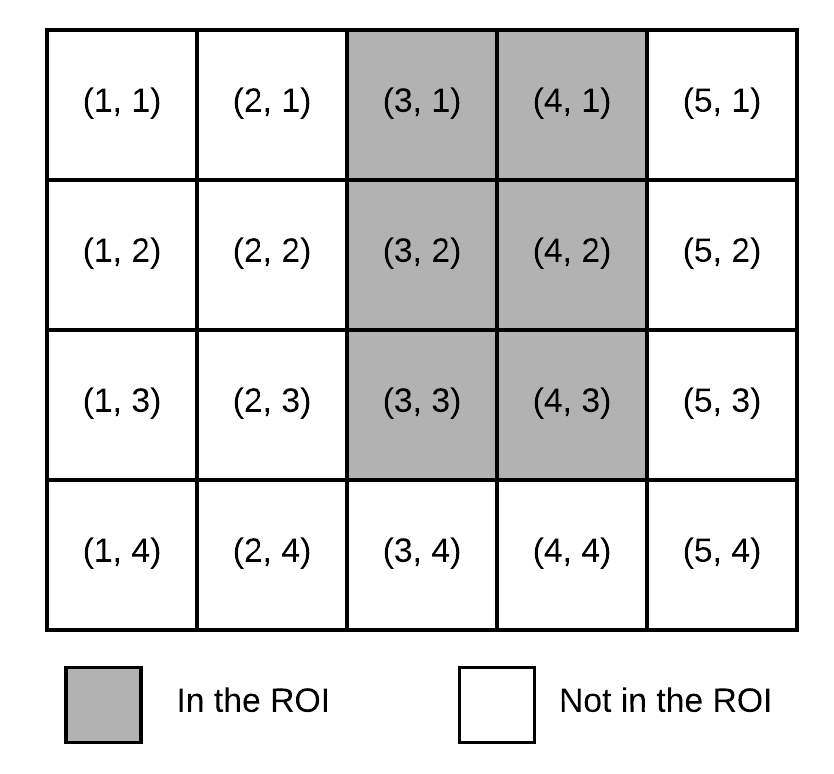
\includegraphics[scale=0.8]{./images/ROI.png}
    \caption{Example of how we may define a ROI in our node. This example features a MSI dataset of width 5 and height 4. The ROI is specified with a minimum  and maximum width of 3 and 4 respectively, and a minimum and maximum height of 1 and 3 respectively.}
    \label{fig:ROI_Image}
\end{figure}

\section{Average and Basepeak Spectra}
McDonnell et al. provide a discussion on data reduction methods for feature identification in MSI data, which is based on the concept of spectral representations \cite{mean_basepeak_spectrum_MSI}. This involves representing the spectra in a multitude of different fashions. Notably, calculating the mean spectrum, and a basepeak spectrum through the following two algorithms. 

% Print mean spectrum calculation

    \begin{algorithm}
        \label{alg:calculate_mean_spectrum}
        \caption{Calculate the mean spectrum.}
        \begin{algorithmic}
            \Require $D$ is the set of all spectra in our dataset, $L$ is the length of spectra in $D$.
            \Ensure $S_{mean}$ the mean spectrum.
           
            \Procedure{MeanSpectrum}{$S,D$}
            
            \State Initialize an array $S_{mean}$ of length L.
            \State $n \gets 0$
            
            \For{Spectrum $S$ in dataset $D$}
                \For{$i := 0$ \textbf{to} $L - 1$}
                \State $S_{mean}[i] = S_{mean}[i] + S[i]$
                \EndFor
                
                \State $n \gets n + 1$
            \EndFor
            
            \For{index $i:=0$ \textbf{to} $i = L - 1$ }
                \State $S_{mean}[i] \gets S_{mean}[i] / n$
            \EndFor
            
            \State \textbf{return} $S_{mean}$
            \EndProcedure
        \end{algorithmic}
    \end{algorithm}


% Print Basepeak spectrum calculation

    \begin{algorithm}
        \label{alg:calculate_basepeak_spectrum}
        \caption{Calculate the Basepeak spectrum.}
        \begin{algorithmic}
            \Require $D$ is the set of all spectra in our dataset, $L$ is the length of spectra in $D$.
            \Ensure $S_{bp}$ the basepeak spectrum.
           
            \Procedure{BasepeakSpectrum}{$S,D$}
            
            \State Initialize an array $S_{bp}$ of length L.
            
            \For{Spectrum $S$ in dataset $D$}
                \For{$i := 0$ \textbf{to} $L - 1$}
                \State $S_{bp}[i] =  \max \{S_{bp}[i], S[i]\}$
                \EndFor
            \EndFor
            \State \textbf{return} $S_{bp}$
            \EndProcedure
        \end{algorithmic}
    \end{algorithm}


The spectra typically have the baseline removed and is smoothed before these spectral representations are calculated, to allow for better results during peak picking phases that occur after.

\begin{figure}[H]
    \centering
    \subfloat[Mean Spectrum][Mean Spectrum]{
        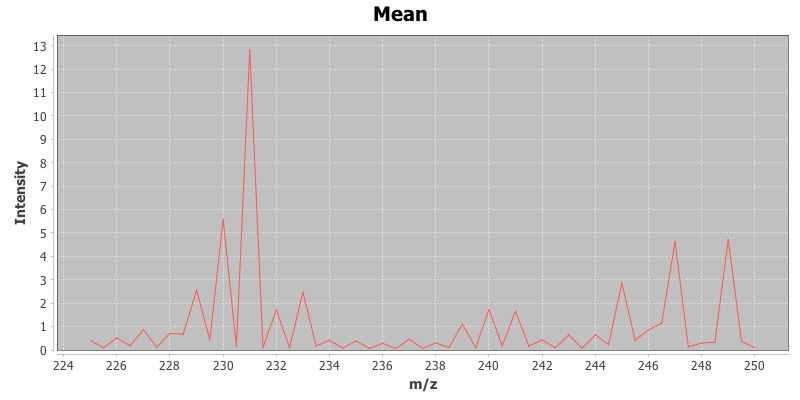
\includegraphics[width=0.7\textwidth]{./images/mean_basepeak/Mean_urinarybladder.jpeg}
        \label{fig:mean_spectrum}
    }
    
    \subfloat[Basepeak Spectrum][Basepeak Spectrum]{
        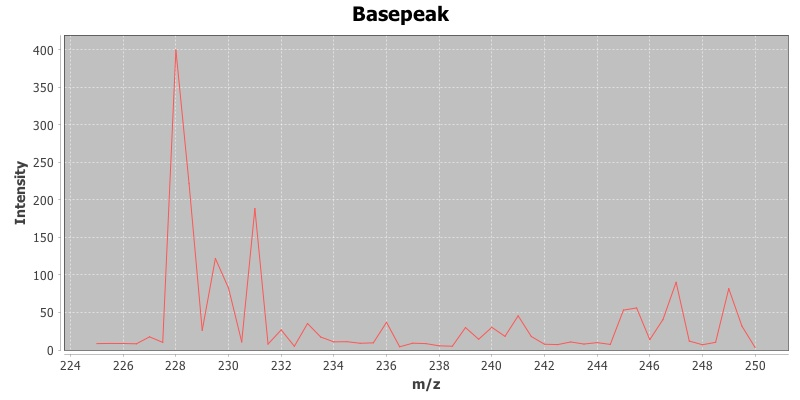
\includegraphics[width=0.7\textwidth]{./images/mean_basepeak/Basepeak_urinarybladder.jpeg}
        \label{fig:basepeak_spectrum}
    }
    \caption{Mean and basepeak spectra of the urinary bladder dataset \cite{imzml.org} that we have seen throughout this report. Before calculating these spectra, the spectra were rebinned, smoothed using a Savitzky-Golay filter, and a minimum baseline was subtracted. As we might expect, the scaling of the intensities of these two line charts is greatly different, the basepeak spectrum requiring a much larger scale as we might expect.}
    \label{fig:mean_basepeak_spectra}
\end{figure}

Race et al. provides an algorithm for memory efficient spectral representation generation \cite{alan_race_phd_thesis}, in which we preprocess each spectra individually, and then update the spectral representation accordingly to the type of spectra being generated. Our software works in a similar way, where we preprocess the dataset in a Knime loop of $k \in \mathbb{N}$ spectra per loop, which on completion connects to the spectral representation node, and again passes through the data. We see that our software relies on two passes of the data, and the algorithm provided needs only one pass of the data. This brings us to a drawback of our system design, in that we sometimes are required to pass through the data more times than necessary with regards to spectral representations, as each Knime node has one specific capability. However we note that our system aims to be easy to use, because of this we saw it as a worthy trade off, as nodes would become too complicated to use if they performed too many tasks, which would be necessary for a single pass of the data and a spectral representation being generated.

\section{Limit m/z Range}
This is the simplest of our preprocessing nodes, it limits our dataset between a minimum and a maximum m/z ratio. The user simply inputs a minimum and maximum m/z, and then all columns containing m/z values outside of that range are deleted and not considered for the rest of the workflow. It does this to both the m/z and their corresponding intensity tables. 

\section{Utility Nodes}
In this section we talk about something which is loosely related to the preprocessing of MS data which we have been talking about previously. That is our category of utility nodes which currently has only one node, but is still a category as it is likely there will be more utility functions required for uor extension. This node is the "Combine m/z and Intensity", which we use to combine the m/z and intensity tables into one \texttt{DataTable}. It is designed to be used when there is a common m/z, and thus uses the first m/z array in the m/z table to create the \texttt{DataTable}'s column header. Then the intensity data is input as rows in the table as normal. We do this as the design of our system requires separate m/z and intensity tables for the preprocessing stage, and then a single table for any later processing, such as clustering and any visualizations. Doing this requires less data throughput in each subsequent node in the workflow, and we expect a common m/z by this stage of the workflow. 

\chapter{Mass Spectrometry Imaging}
Imaging is a fundamental part of MS, typically done in the later stages of a workflow. There are two main ways in which we can visualize Mass Spectrometry data. The first of which is plotting individual spectra with their m/z values as the x axis, and the intensity values as the y axis. Secondly, we can build images at specific m/z channels, where we assign a colour to every pixel in the image equal to its intensity value at the m/z channel of interest. We note that if we use a loop end node, it will automatically add an iteration column to the end of the output DataTable. For our visualization nodes to work we must change this setting on the respective Loop End node, so that no iteration column is appended. In this chapter, we will look at the nodes that we have implemented that can be used to create visualizations of MSI data. 

\section{Spectrum Viewer}
The node that we have implemented for visualizing single spectra takes on input $x \in \mathbb{N}$ and $y \in \mathbb{N}$. It then searches for a value in the DataTable  which has a row key with unique identifier $(x,y)$. It then proceeds to create a chart plotting the m/z values, which are the column names of the DataTable, against the intensity values present in that row. Note, that if either $x$ or $y$ values on input are greater than the size of the image, it simply finds the closest possible spectrum. We see examples of this throughout the report, here is one example in figure \ref{fig:example_spectra_viewer}. We used the JFreeChart 1.0.19 java library to build, display, and save to a specified directory these line charts of spectra. There is a separate node that we have created, which is exactly the same as this node, except that instead of displaying, it saves every spectra, thus it is most suitably used when reading imzML in chunks of data, to save the images between preprocessing nodes. However, this is quite costly with regards to efficiency, and so in general is not recommended, especially for large datasets, we recommend only saving and looking at important spectra.

\begin{figure}
    \centering
    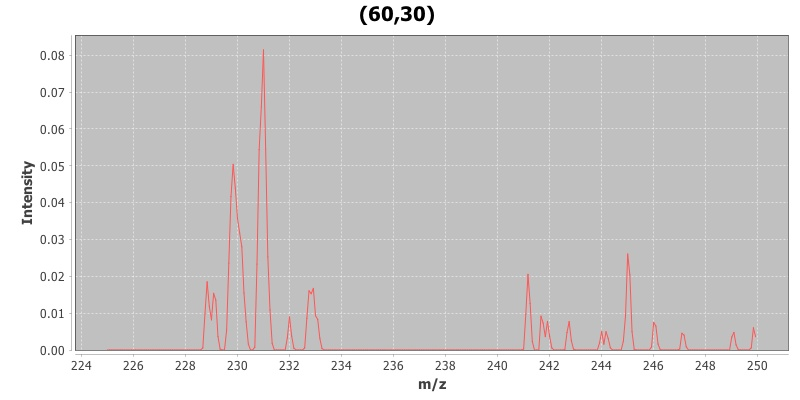
\includegraphics[width=\textwidth]{./images/MS_Imaging/(60,30)_urinarybladder_smooth_normalize.jpeg}
    \caption{Example of a spectra of location (60,30) from the urinary bladder dataset \cite{imzml.org}, it has been smoothed using a Savitzky-Golay filter, and then normalized using the Total Ion Count. We see a group of peaks with high intensity in the m/z range of 228 to 234, and then smaller peaks in the m/z range 241 to 247.}
    \label{fig:example_spectra_viewer}
\end{figure}

\section{Spectrum Viewer (Compare)}
Similar to the Spectrum Viewer, we have added a node that is used to sketch multiple spectra in one image, so that they can be easily compared. The node uses that same functionality as the Spectrum Viewer node, however it takes on input multiple x and y values. We see an example of this where three spectra are plotted in figure \ref{fig:MS_Imaging:multiple_spectra_example}.

\begin{figure}
    \centering
    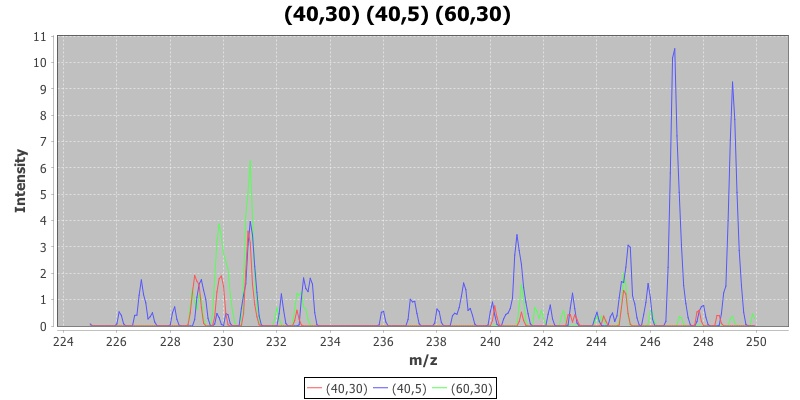
\includegraphics[width=\textwidth]{./images/MS_Imaging/(40,30)-(40,5)(60,30)-urinarybladder_smooth.jpeg}
    \caption{Example of three spectra plotted into the same line chart. The pixel locations of the spectra plotted are (40,30), (40,5), (60,30). We see that the (40,30) and (60,30) share common peak locations, as does (40,5) which has more peaks where the others have none.}
    \label{fig:MS_Imaging:multiple_spectra_example}
\end{figure}

\section{m/z Channel Viewer}
The m/z channel viewer creates images over the entire space of the dataset, more specifically, we specify an m/z chennal $m \in \mathbb{R}^{+}$, and then we get the intensity value of each location in the image at that m/z. Next, we assign a value to the intensity which can then translate to a color in the image. For the purpose of this project, we deal with grayscale images, and thus assign pixel values of between 0 and 255. We calculate a maximum intensity which can be a local maximum or a global maximum, where the local maximum is the largest value in the specified m/z channel, and a global maximum is the highest value found in the entire dataset for any m/z value. We scale it using the following,

\begin{equation}
    \centering
    \label{eqn:scale_pixel_value}
    P_{i,j} = (I_{i,j} \text{ div } max) \cdot 255.
\end{equation}

In this equation, $i$ and $j$ refer to the spatial location of the pixel, $P_{i,j} \in {0, 1, \dots 255}$ is the pixel value, and $I_{i,j}$ is the intensity value of the pixel at the m/z of interest. The full algorithm, which requires only one spectrum in memory at any given time is documented in algorithm 8. We use the imglib2 library to build the m/z channel image from the calculated pixel array, imglib2 is the general purpose image processing library that ImageJ2 is built upon \cite{imglib2}.

% Get the intensity Array.
\begin{algorithm}
    \caption{Calculate the grayscale pixel array.}
    \begin{algorithmic}
        \Require $D$ is the table of MSI data, with spectra sorted by pixel location as rows in the table. $m \in \mathbb{R}^{+}$ is the m/z channel.
        \Ensure $P$ is the pixel array of values with m/z equal to $m$.
           
        \Procedure{CalculatePixelArray}{$D,m$}
            \State Initialize array $P$ with length $n$, where $n$ is the number of pixels.
            \State $tmp \gets 0$
            \For{Spectrum $S$ in $D$}
                \State $P[tmp] \gets S[m]$
                \State $tmp \gets tmp + 1$
            \EndFor
            
            \State $max \gets $ maximum value in $I$ \textbf{OR} $D$.
            
            \For{$i := 0$ \textbf{ to } $n - 1$}
                \State $P[i] \gets (P[i] \text{ div } max) \cdot 255$
            \EndFor
            \State \textbf{return} $P$
        \EndProcedure
        \end{algorithmic}
        \label{alg:calculate_intensity_array_for_mz_image}
    \end{algorithm}
    
\begin{figure}
    \centering
    
\includegraphics[width = \textwidth]{./images/ion_images/urinarybladder_ion_image_mz240_08.png}
    \caption{An ion image of the m/z channel with a local maximum intensity at m/z channel 240.08, generated by our software. The dataset is 180 by 90 pixels and thus we have scaled this image accordingly.}
    \label{fig:ion_image_240.08}
\end{figure}

\begin{figure}
    \centering
    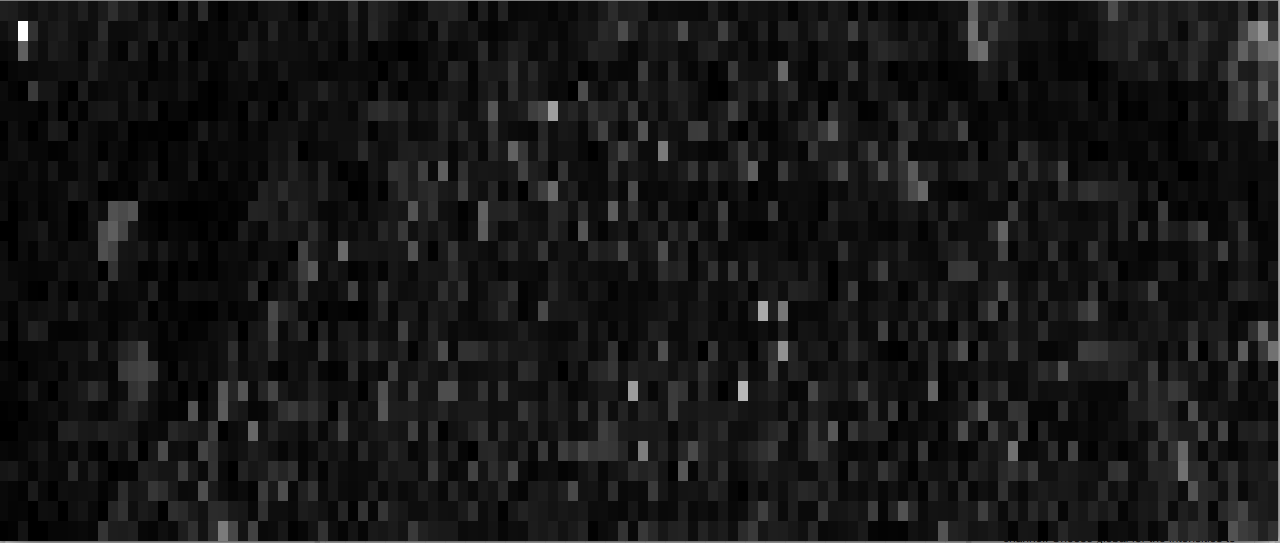
\includegraphics[width = \textwidth]{./images/ion_images/urinarybladder_ionimage_mz231.png}
    \caption{An ion image of the m/z channel with a local maximum intensity at m/z channel 231.08, generated by our software. The dataset is 180 by 90 pixels and thus we have scaled this image accordingly.}
    \label{fig:ion_image_231}
\end{figure}
    
\section{Cluster Viewer}
The last of our visualization nodes is used to display the values achieved from applying clustering techniques to our data. The Knime standard for clustering nodes is to return the original, incoming data but with a new column appended, which is of type string, and contains values of the form "cluster\_x", where $x \in \mathbb{N}$ is the cluster value that the row belongs to. Thus we build the cluster array by parsing the cluster values from this column, and then the pixel array is calculated in a similar fashion to the m/z channel viewer. We create a grayscale image where the pixels are scaled to the number of clusters.


\chapter{Clustering MS}
As we have seen, Mass Spectrometry data is extremely noisy, and there are multiple different types of noise appear for different reasons. We can denoise our data, and then apply various clustering algorithms, in the hope that we can view natural groupings between spectra an their spatial locations. 

\section{Normalized Cuts}
Normalized cuts is a recursive, graph based image segmentation algorithm originally proposed by Jianbo Shi and Jitendra Malik. The algorithm returns a hierarchical set of partitions of data, the clusters, and aims to partition "\textit{from the big picture downwards, like a painter first marking out major details and then filling in details}" \cite{normalized_cuts_algorithm}. Normalized Cuts is well suited towards MSI data and imaging in general as it not only considers the features in a data point, but also their spatial location, so points closer together achieve a higher similarity score. In these next few paragraphs we will aim to give a general overview as to how the algorithm works, and we will give an in detail look at how we have implemented this algorithm for use in MSI data.

The first step in the algorithm is to build the weighted, undirected graph which we use to represent our data points, $G = (V, E)$. V is the set of vertices in $G$, which is every data point in $G$, and $E$ is the set of edges in $G$, which connects every $v \in V$ together. We summarize this graph by creating a similarity matrix $\mathbf{W} = [w_{i.j}]$, which is a sparse symmetric matrix where $w_{i,j}$ is the weight of the edge between vertices (typically pixels) for every $i,j \in V$. We assign a value to each $w_{i,j}$ using the following 

\begin{equation}
    w_{i,j} = \exp{ \frac{ -{|| F(i) - F(j) ||}_2^2 }{ \sigma_I }   }  \cdot 
        \begin{cases}
        \exp{ \frac{ -{|| X(i) - X(j) ||}_2^2 }{ \sigma_X }   } & \text{if } || X(i) - X(j) ||_2 < r,\\ 
        0 & \text{otherwise},
        \end{cases}
    \label{equation:norm_cuts_assign_weight_w_ij}
\end{equation}

where $X(i)$ refers to the spatial location of the vertex $i$, $F(i)$ refers to a feature vector assigned to the vertex $i$, these can depend on the implementation of the algorithm. The terms $sigma_I, sigma_X, r \in \mathbb{R}^{+}$ are all parameters which can affect the output of the algorithm. We can view the piecewise term above as the spatial factor for $w_{i,j}$, and the initial term as the feature factor for $w_{i,j}$, the $sigma_I$ and $sigma_X$ terms scale the effect of their respective factor, meanwhile the $r$ term determines how far away points must be with regards to their spatial location to deserve a weight of 0, and thus it determines the sparsity of our weight matrix $\mathbf{W}$.

Once the weight matrix is calculated, we begin partitioning. We aim to partition the graph into two subsets of $V$ that can be rebuilt into graphs $A,B$ such that $A \cup B = V$, and $A \cap B = \emptyset$. We measure the degree of dissimilarity between these bipartitions by calculating $cut(A,B)$, and an optimal bipartition for these sets $A,B$ minimise this value. However, it is well documented that the minimal cut calculates a biased bipartitions $A,B$ such that one of $A$ or $B$ are small set of points in the graph \cite{normalized_cuts_algorithm}. This is clearly not appropriate as we have seen that the algorithm aims to work from large global partitions to smaller subpartitions. This is where Normalized Cuts receives its name, as Jianbo Shi and Jitendra Malik introduce a new measure of dissimilarity, which aims to decrease the effect of this bias, the normalized cut or $Ncut$.

\begin{equation}
    Ncut(A,B) = \frac{cut(A,B)}{assoc(A,V)} + \frac{cut(A,B)}{assoc(B,V)}
    \label{equation:Ncut_equation}
\end{equation}

The $assoc(A,V)$ is the sum of weights of the edges in $A$ that are connected to the graph. Now we are required to calculate the partition which minimizes the $Ncut$. Jianbo Shi and Jitendra Malik give an extensive proof that gives us the following \cite{normalized_cuts_algorithm},

\begin{equation}
    \min_x Ncut(x) = \min_y \frac{ \mathbf{y}^T (\mathbf{D} - \mathbf{W}) \mathbf{y} }{ \mathbf{y}^T \mathbf{D y} }.
    \label{equation:n_cuts_to_raleigh_quotient}
\end{equation}

Here, $\mathbf{D}$ is a diagonal matrix, which is the same size as $\mathbf{W}$, and the diagonal entries are $d_{i,j} = \sum_j w_{i,j}$ for all $i=j$.  However, the right hand side is a Rayleigh quotient and we can transform it to the following.

\begin{equation}
    (\mathbf{D} - \mathbf{W}) \mathbf{y} = \lambda \mathbf{D} \mathbf{y}
    \label{equation:general_eigenvalue_problem}
\end{equation}

This can be then simplified to the following standard eigenvalue problem to be solved more easily.

\begin{equation}
    \mathbf{D}^{-\frac{1}{2}} (\mathbf{D} - \mathbf{W}) \mathbf{D}^{-\frac{1}{2}}  x = \lambda x.
    \label{equation:standard_eigenvalue_problem}
\end{equation}

$(\mathbf{D} - \mathbf{W})$ is the Laplacian matrix, and $x = \mathbf{D}^{\frac{1}{2}} \mathbf{y}$. We can easily verify that a solution to this eigenvalue problem is $x_0 = \mathbf{D}^{\frac{1}{2}} \mathbf{1}$. We are shown that the optimal solution to minimizing the $Ncut$ is the second eigenvector of the above standard eigenvalue system in equation \ref{equation:standard_eigenvalue_problem}.

We partition the second eigenvector into two subgraphs in one of three ways. The first two involve a splitting value which is either zero or the median of the eigenvector. Then all indices with eigenvector values less than the splitting value are added to partition $A$, all others belong in partition $B$. We then run the algorithm again on each bipartition until a constraint breaks and we cannot recursively call it again, for example a maximum number of clusters reached. The other approach is to estimate the bipartition which minimizes the $Ncut$, by using the following algorithm. 

% Partition the eigenvector.
\begin{algorithm}
    \label{alg:calculate_ncut_bipartition}
    \caption{Estimate the bipartition which minimizes the $Ncut$ value.}
    \begin{algorithmic}
        \Require $v$ is the second eigenvector of our standard eigenvalue problem in equation \ref{equation:standard_eigenvalue_problem}. $l \in \mathbb{R}^{+}$ is the accuracy to which we estimate the bipartition.
        \Ensure $A$ and $B$ which are disjoint sets of all the indices in v such that $A \cup B = V$ and $A \cap B = \emptyset$.
        \Procedure{EstimateOptimalBipartition}{$v, l$}
            
        \State $m \gets \min \{v[i] \text{ }| \text{ } i \text{ is a valid index in v.}\}$
        \State Initialize a list $cuts$.
        \State $b \gets true$
            
        \While{b == true}
            
            \State Initialize lists $p_1$ and $p_2$
            \For{index $i$ in $v$}
                    
                \If{$v[i] < m$}
                    \State add $i$ to $p_1$
                \Else
                    \State add $i$ to $p_2$
                        
                \EndIf
            \EndFor
            
            \State add $NCut(p1,p2)$ to the list $cuts$
            
            \If{$p_2$ contains 0 elements}
                \State b = false
                \State \textbf{break}
            \EndIf
            
            \State $m = m + l$
                
        \EndWhile
            
        \State sort the list cuts from smallest to largest.
        \State $best \gets v[0]$
            
        \State Create set $A$ containing indices of $v$ where $v[i] < best$
        \State Create set $B$ containing indices of $v$ where $v[i] \geq best$
            
        \State \textbf{return} A and B
        
        \EndProcedure
    \end{algorithmic}
\end{algorithm}

\subsection{Application to MSI}
We have chosen to implement our Normalized Cuts algorithm in a way that allows us to easily extend it's logic and alter the implementation so that it will work for any specific use case. We have done this by creating a main java class NormalizedCuts, which is an abstract java superclass that stores all the logic that is general to the Normalized Cuts algorithm. In order to inherit this logic, we create a class which extends NormalizedCuts. This requires us to implement the three following methods :


\begin{itemize}
    \item setSimilarityMatrix() - which is used to set the similarity matrix $\mathbf{W}$.
    \item getWeight() - which is used to set the weight value between two spatial locations $i$, and $j$.
    \item getFeatureFactor() - which is used to assign the notion of similarity between two $i$ and $j$, as seen in equation \ref{equation:norm_cuts_assign_weight_w_ij}.
\end{itemize}

Here we will talk about how we have implemented the Normalized Cuts algorithm to work for MSI data. We assign the similarity matrix such that every spatial location, or pixel, in the MSI dataset receives a column and a row in the weight matrix $\mathbf{W}$. As we know the matrix $W$ is symmetric, we only calculate the weights between pixels $i$ and $j$ in the upper triangle of the matrix, but set both $w_{i,j}$ and $w_{j,i}$ equal to their weight. In our implementation to be used for MSI data, we calculate the $F(i) - F(j)$, as seen in equation \ref{equation:norm_cuts_assign_weight_w_ij} by the following,

\begin{equation}
    F(i) - F(j) = S_i [m] - S_j[m].
\end{equation}

Where $S_i$ is the spectrum associated with pixel $i$ and $S_j$ is the spectrum associated with $j$, for every valid index $m$ in the spectra. Lastly, we must calculate the spatial part of this equation, which is given by $X(i) - X(j)$ in equation \ref{equation:norm_cuts_assign_weight_w_ij}, which is done by the following,

\begin{equation}
    X(i) - X(j) = [x_i, y_i] - [x_j, y_j].
\end{equation}

Every spatial location $i$ will have an associated pixel, with its location in the original image as $(x_i, y_i)$, where the $x_i$ shows the pixels location in the width of the image, and $y_i$ of course is the location in the height of the image. 

\begin{algorithmic}
    \label{alg:recursiveCut_ncuts}
    \begin{algorithm}
        \caption{Recursive Cut method for Normalized Cuts, cut matrix $\mathbf{W}$ into two partitions.}
        \Require List of BiPartitions $P$ with their respective similarity matrix $\mathbf{W}$, the NCut threshold value $\gamma$.
        \Ensure Recursively cut the Partition P.
        
        \Procedure{RecursiveCut}{$P, \gamma$}
        
            \For{Partition $P_i$ and similarity matrix $\mathbf{W}_i$ \textbf{ in } $P$}
                \State Calculate $\mathbf{D}$ from $\mathbf{W_i}$
                \State Calculate $\mathbf{D}^{1/2}$
                \State $\mathbf{E} \gets \mathbf{D}^{-\frac{1}{2}} (\mathbf{D} - \mathbf{W}) \mathbf{D}^{-\frac{1}{2}}$
                \State $v_2 \gets $ Second Eigenvector of $\mathbf{E}$
                \State \textbf{call} EstimateOptimalBipartition() to get optimal partitions $A,B$ from $v_2$
                \State $\gamma_{P_i} \gets NCut(A,B)$ 
                
                \If{$\gamma_{P_i} > \gamma$} \Comment{No suitable partitions.}
                    \State \textbf{continue}
                \EndIf
            
                \If{size of $A \geq 2$}
                    \State \textbf{call} recursiveCut$(A, \gamma)$
                \EndIf
                \If{size of $B \geq 2$}
                    \State \textbf{call} recursiveCut$(B, \gamma)$
                \EndIf
            \EndFor
        \EndProcedure
    \end{algorithm}
\end{algorithmic}

\subsection{Lanczos Algorithm}
We notice that in order to perform Normalized Cuts, we are required to calculate the second eigenvector of extremely large matrices. Inparticular, if there are $n \in \mathbb{N}$ pixels in an image, then we will create a similarity matrix of size $n \times n$. We can perform the Lanczos algorithm to approximate extreme eigenvalues and eigenvectors to speed this up. Lanczos makes use of more efficient eigendecomposition of tridiagonalized matrices \cite{normalized_cuts_algorithm}.

 
    \begin{algorithm}
        \label{alg:lanczos}
        \caption{Calculate extreme eigenvectors and eigenvalues of matrix $\mathbf{A}$ efficiently.}
        \begin{algorithmic}
        
            \Require Symmetric Matrix $\mathbf{A} \in \mathbb{R}_{n,n}$, $k \in \mathbb{N}$ is the eigenvalue eigenvector pair we wish to calculate.$l$ is the accuracy, $m \in \mathbb{N}$ is the max number of Lanczos iterations if we haven't found an accurate estimate.
            \Ensure The k-th eigenvalue and eigenvector.
           
            \Procedure{Lanczos}{$\mathbf{A},k$}
         
            \State Initialize three lists $alphas, betas, V$.
            \State $n \gets $ width or height of matrix $\mathbf{A}$.
            \State Generate a random unit vector $\mathbf{v}$ which has $n$ elements.
            \State Add $\mathbf{v}$ to the list $V$.
            
            \State $\mathbf{w}^{'} \gets \mathbf{A} \mathbf{v}$ 
            \State $\alpha \gets \mathbf{w}^{'} \cdot \mathbf{v}$
            \State Add $\alpha$ to the list $alphas$
            \State $\mathbf{w} \gets \mathbf{w}^{'} - \alpha \mathbf{v}$
            
            %\State Declare variable $eigval$
            %\State Declare variable $eigvec$
            
            \For{i := 2 \textbf{to} m}
            
                \State Add $||\mathbf{w}||$ to the list $betas$. 
                
                \If{$betas[i-1] \neq 0$}
                    \State $\mathbf{v} = \frac{1}{betas[i-1]}\mathbf{w}$
                    \State Add v to the list $V$
                \Else
                    \State \textbf{throw} Exception("$\beta = 0$.")
                \EndIf
                
                \State $\mathbf{w}^{'} \gets \mathbf{A}\mathbf{v}$
                \State Add $\mathbf{w}^{'} \cdot v$ to the list $alphas$
                \State $\mathbf{w} \gets \mathbf{w}^{'} - alphas[i] \cdot \mathbf{v} - betas[i - 1] \cdot V[i-1] $
                
                \State Make matrix $V_m$ where the vectors in list $V$ are columns in the matrix.
                \State Create tridiagonal matrix $\mathbf{T}$ with $alphas$ as the diagonal and $betas$ the diagonal above and below.
                
                \State Eigendecompose $\mathbf{T}$ to get the k-th eigenvector $t_i$ and eigenvalue $\lambda_i$.
                
                \If{$t_i$ is sufficiently close w.r.t accuracy $l$}
                    \State $i \gets m + 1$
                \EndIf
            \EndFor
        
            \State \textbf{return} The k-th eigenvalue and eigenvector $\mathbf{t}$ and $\lambda$.
            \EndProcedure
        \end{algorithmic}
    \end{algorithm}
    
\subsection{Limitations}
Our software implementation uses the apache-commons matrix library. There is a limit on the size of these matrices, even when sparse, meaning that the maximum image size we can operate the algorithm on is 215 x coordinates and 215 y coordinates.  

\begin{figure}
    \centering
    \subfloat[k-means performed on a basic synthetic dataset.][k-means performed on a basic synthetic dataset.]{
    
\includegraphics[width=0.3\textwidth]{./images/cluster/k_means_cluster_image.png}
    }
    \subfloat[Normalized cuts performed on a basic synthetic dataset, shows poor results when the incorrect parameters are passed, with improved parameters we get input similar to k-means.][Normalized cuts performed on a basic synthetic dataset, shows poor results when the incorrect parameters are passed, with improved parameters we get input similar to k-means.]{
    
\includegraphics[width=0.3\textwidth]{./images/cluster/Norm_Cuts_Img.png}
    }
    
    \caption{We perform some clustering on some basic synthetic data of 100 spectra, with a spatially defined structure which was captured exactly by k-means.}
    \label{synthetic_data}
\end{figure}

The Normalized Cut algorithm is quite particular about the input parameters $\sigma_I, sigma_X, r$ and the Lanczos accuracy that is used. Getting poor results if the accuracy is low, in particular when we choose to measure eigenvalues instead of eigenvector coefficients to see how close the Lanczos approximation is getting, see \ref{synthetic_data}.

\section{Other Clustering Algorithms}
We ahve provided an implementation of Self Organizing Maps (SOM) using the javaML library, and saw that it worked well with small synthetic MSI datasets. Knime implements k-means and DBSCAN in the node repository.

%-----------------------------------------------------------------------
% SECTION : SUMMARY & CONCLUSIONS
%-----------------------------------------------------------------------
\chapter{Summary and Future Work}
In this chapter, we will discuss the possibilities of further work that can be done in extending the software extension that we have implemented and conclude the report.

\section{Future Work}
We have seen that peak detection and peak alignment provide important results when performed on spectral representations \cite{msi_data_spectral_representations}. I believe that this work would be an interesting route to take. Furthermore, I believe that the visualization techniques provided by MSIQuant and Spectral Analysis \cite{spectral_analysis_article} \cite{MSI_QUANT_Article} are superior to ours, and they could provide some inspiration as to future work we can perform.

Some excellent work in the future could include the implementation of topological clustering algorithms, in particular ToMaTo as proposed in \cite{chazal2013persistence}. This could also give rise to new peak detection algorithms also. Perhaps once that is finished, a more quantitative analysis of the clustering algorithms could be performed using synthetic spectra, which would give a big improvement to this piece of work.

\section{Conclusion}
In this project we aimed to create a software extension that is extensible, open source, supports a common data format, and is easy to use.  We also aimed to explore clustering techniques that are used in MS. This project has been challenging, and we believe that the software implementation of preprocessing and visualization methods has been quite successful. In particular we have explored the use of Baseline subtraction methods and found that the morphological operators work very well. However, there is room for improvement with regards to this project and the software implementation and evaluation of clustering algorithms used in MS, in particular topological clustering would be of great interest in this domain.

%-----------------------------------------------------------------------
% Print the Bibliography
%-----------------------------------------------------------------------
%\nocite{*}
\printbibliography[heading=bibintoc,title={Bibliography}]

%-----------------------------------------------------------------------
% APPENDICES
%-----------------------------------------------------------------------
\chapter*{Appendix}
\addcontentsline{toc}{chapter}{Appendix}

\subsection*{Version Control}
All of the source code that was developed in this project, weekly logs and meeting notes can be found in the git repository with the following url, \url{https://git-teaching.cs.bham.ac.uk/mod-msc-proj-2017/apt467/}. Source code that was developed for our software extension of Knime is all placed in the directory "knime\_dev/MassSpectInKnime". Source code that was created for the implementation of Normalized Cuts was implemented in the directory "knime\_dev/NormalizedCuts2". We see that there are several directories named "week\_x", which contain useful information about what was done in that given week of the project. In the root directory of our git repository is a .jar file, which is the latest version of our software. There is a subdirectory containing information regarding the report and the presentation.

\subsection*{How to use the software}
In order to use this software, download the latest version of Knime which can be found with the following url, \url{https://www.knime.com/downloads/download-knime}. In the root of our git repository specified above, we can find the latest version of our software built into a .jar with the name "MassSpectInKnime2\_1.0.1.jar". To use this jar in Knime, we must copy it to the following location in your installed Knime application, "My\_Knime/Contents/Eclipse/dropins/". Note that you must restart your Knime application for our extension to appear. Once you start the Knime application, you will see our category of nodee at the bottom of the node repository. The Normalized Cuts algorithm can be used in the directiory "knime\_dev/NormalizedCuts2".

\subsection*{Supporting Information}
\label{subsection:Appendix/Supporting_Information}
Here is a view only link to the google docs which stores the supporting information for our software extension, \url{https://docs.google.com/document/d/1qubH8Fj5ZBY\_dTpSzsnP7bkGbMytSwhDUNBJUgyGnJ4/edit?usp=sharing}. Note that as of handing in this report, this document is not fully completed and is a work in progress. 


\end{document}


%-----------------------------------------------------------------------------
% Here is documentation about the LaTeX template that I am using.
%-----------------------------------------------------------------------------

%%%%%%%%%%%%%%%%%%%%%%%%%%%%%%%%%%%%%%%%%
% University Assignment Title Page 
% LaTeX Template
% Version 1.0 (27/12/12)
%
% This template has been downloaded from:
% http://www.LaTeXTemplates.com
%
% Original author:
% WikiBooks (http://en.wikibooks.org/wiki/LaTeX/Title_Creation)
%
% License:
% CC BY-NC-SA 3.0 (http://creativecommons.org/licenses/by-nc-sa/3.0/)
% 
% Instructions for using this template:
% This title page is capable of being compiled as is. This is not useful for 
% including it in another document. To do this, you have two options: 
%
% 1) Copy/paste everything between \begin{document} and \end{document} 
% starting at \begin{titlepage} and paste this into another LaTeX file where you 
% want your title page.
% OR
% 2) Remove everything outside the \begin{titlepage} and \end{titlepage} and 
% move this file to the same directory as the LaTeX file you wish to add it to. 
% Then add \input{./title_page_1.tex} to your LaTeX file where you want your
% title page.
%
%%%%%%%%%%%%%%%%%%%%%%%%%%%%%%%%%%%%%%%%%
%\title{Title page with logo}
%----------------------------------------------------------------------------------------
%	PACKAGES AND OTHER DOCUMENT CONFIGURATIONS
%----------------------------------------------------------------------------------------